


\subsection{Why be Bayesian?}\label{Why Bayesian}
When we first encounter statistical modelling, we often focus on finding the “best parameter estimate,” such as using Maximum Likelihood Estimation (MLE), the Method of Moments, or Least Squares regression as common non-Bayesian approaches to fit the model to the data~\cite{van2021bayesian}. This works well in many tasks, but in practice, we also need to know how uncertain that estimate is~\cite{gelman1995bayesian}. 

In situations with a limited sample size, complex structures, or high censoring rates, classical estimators can be biased, and their uncertainty is hard to quantify~\cite{van2021bayesian, ibrahim2013bayesian}. For example, in Efron’s leukemia survival study~\cite{Efron01091977}, only $21$ patients were included, and over half were right-censored. The Cox model estimated a hazard ratio of about $2.0$, but with a standard error nearly as significant as the estimate, giving a wide 95\% CI ($\approx$0.8–5.0) and making risk assessment unreliable. This illustrates how high censoring and small samples can destabilise classical estimators, a challenge frequently encountered in survival studies where censoring may be driven by complex or partially unobserved mechanisms. Such situations are difficult for classical methods but naturally handled in a Bayesian framework.

Bayesian methods address this limitation by treating parameters as random variables whose uncertainty is described by a probability distribution~\cite{gelman1995bayesian}. This allows prior information and data evidence to be combined through
$$
\text{Posterior}(\theta \mid data)
\propto
\text{Likelihood}(data \mid \theta)
\times
\text{Prior}(\theta),
$$
yielding a full posterior distribution rather than a single estimate. This reframes inference from “finding the right number” to dynamically updating and refining beliefs, providing not only point estimates but also credible intervals and posterior predictive distributions for a complete picture of uncertainty~\cite{gelman1995bayesian}.

The flexibility of this approach makes it applicable from simple mean estimation and regression to hierarchical, time-series, and deep generative models~\cite{carlin1997bayes}. In survival analysis, where censoring is common, Bayesian models naturally accommodate it within the likelihood~\cite{bartovs2022informed}. When sample sizes are small or censoring rates are high, priors can stabilise estimation by incorporating historical data or expert knowledge~\cite{gelman1995bayesian}. Whether using parametric or non-parametric approaches, Bayesian inference offers a structured, interpretable, and extensible framework~\cite{van2021bayesian}. 

Later in this study, we will build on this Bayesian foundation to introduce modelling extensions that explicitly account for censoring mechanisms, allowing us to address limitations of standard survival models in a principled way.




\subsection{Fundamentals of Survival Analysis} \label{Fundamentals of Survival Analysis}
Given the limitations of classical methods discussed in the previous section, particularly under high censoring and small sample sizes, we adopt a Bayesian framework for survival analysis. Before introducing the proposed model, we briefly review the core quantities in survival analysis, which will serve as the foundation for our methodological development~\cite{kleinbaum1996survival}.

In survival analysis, let the true event time for subject $i=1,\dots,n$ be the random variable $T_i\ge 0$. Assume
$$
T_1,\ldots,T_n \stackrel{\text{i.i.d.}}{\sim} F_T,\qquad \text{support }[0,\infty).
$$
If right censoring is present, introduce a censoring time $C_i\ge 0$ and adopt the independent censoring assumption~\cite{kalbfleisch2002statistical}: for each $i$, $T_i\perp C_i$, and observations are independent across subjects; the actually observed data are
$$
Y_i=\min(T_i,\;C_i),\qquad \delta_i=\mathbf 1\{T_i\le C_i\}.
$$
The basic functions that describe the distribution of $T$ are:
\begin{enumerate}
    \item \textbf{Survival function}, the probability that the event has not occurred after time $t$
   \begin{equation}
       S_T(t)=\mathbb P(T>t)=1-F_T(t),\qquad t\ge 0,
   \end{equation}
   where $F_T(t)=\mathbb P(T\le t)$. The function $S_T(\cdot)$ is non-increasing in $t$, is typically taken to be right-continuous, and satisfies $S_T(0^-)=1$~\cite{ibrahim2013bayesian}.
   \item \textbf{Probability density function (PDF)}, the instantaneous density of failure at time $t$ (when $F_T$ is absolutely continuous with respect to Lebesgue measure)
   \begin{equation}
   f_T(t)=\frac{d}{dt}F_T(t)=-\frac{d}{dt}S_T(t)
  \end{equation}
\noindent\textit{Holds at differentiable points / almost everywhere}~\cite{ibrahim2013bayesian,kleinbaum1996survival}.
   \item \textbf{Hazard function}, defined by
   \begin{equation}
        h_T(t)=\lim_{\Delta\downarrow 0}\frac{\mathbb P\big(t\le T<t+\Delta\ \big|\ T\ge t\big)}{\Delta}
          =\frac{f_T(t)}{S_T(t)}\quad(\text{when }S_T(t)>0),
   \end{equation}
   which quantifies the instantaneous failure rate given survival up to $t$~\cite{kalbfleisch2002statistical, ibrahim2013bayesian}. Define the cumulative hazard \begin{equation}
       H_T(t)=\int_0^{t} h_T(u)\,du.
   \end{equation}
\end{enumerate}

Their relationships (under the usual regularity conditions~\cite{kleinbaum1996survival}: $S_T(t)$ is positive, continuous and differentiable on its domain; $h_T(t)$ is locally integrable; and $H_T(t)$ is finite for all $t$) are
\begin{equation}
    f_T(t)=h_T(t)\,S_T(t),\qquad
S_T(t)=\exp\!\Big(-\!\int_0^{t} h_T(u)\,du\Big)=\exp\!\big(-H_T(t)\big),
\label{eq:4}
\end{equation}
and, at differentiable points,
\begin{equation}
    h_T(t)=-\frac{d}{dt}\log S_T(t).
\end{equation}
These three functions are mathematically redundant. Knowing one determines the others, but having all of them is useful for interpretation and application~\cite{kalbfleisch2002statistical}.





\subsection{Parametric Exponential Model} \label{Exponential Model}
%%%%Bridge
In the previous section, we introduced the general setup of survival analysis and the motivation for Bayesian inference. Here, we take the exponential model as a worked example because its simplicity and closed-form properties make it easier to focus on the role of the censoring mechanism without additional model complexity~\cite{kalbfleisch2002statistical, lawless2011statistical}. This clarity will be useful later when introducing an observation-window parameter $A$ to examine its influence on the censoring structure. 

%%%General survival likelihood and Bayesian formulation
\subsubsection{General Survival Likelihood and Bayesian Formulation}
In general, for any parametric survival model with density $f_T(t\mid\theta)$ and survival function $S_T(t\mid\theta)$, the likelihood is
\begin{equation}
L( D \mid \theta)
= \prod_{i=1}^n
\big[ f_T(y_i \mid \theta) \big]^{\delta_i}
\big[ S_T(y_i \mid \theta) \big]^{1 - \delta_i},
\label{eq:8}
\end{equation}
where $\delta_i=1$ indicates an observed event for subject $i$ (contributing $f_T(y_i\mid\theta)$) and $\delta_i=0$ indicates right-censoring (contributing $S_T(y_i\mid\theta)$). Here $y_i$ denotes the observed time $Y_i=\min(T_i,C_i)$~\cite{ibrahim2013bayesian}. 

This formulation coherently combines exact failure times and censored observations under the independent censoring assumption, forming the basis for frequentist estimation approaches and, in the Bayesian framework, being further combined with a prior to yield the posterior distribution~\cite{kalbfleisch2002statistical}.

In the Bayesian framework, the likelihood is combined with a prior $\pi(\theta)$ to form the (unnormalized) posterior
\begin{equation}
\pi(\theta \mid D)
\propto
L(D \mid \theta)\times \pi(\theta),
\end{equation}
which can then be summarised through posterior means, medians, credible intervals, or used for posterior predictive checks~\cite{ibrahim2013bayesian}. The prior $\pi(\theta)$ can be weakly informative (e.g., $\pi(\theta) \propto 1$) or informative, incorporating prior studies or expert knowledge~\cite{carlin1997bayes}. This general formulation applies to any survival model and provides the foundation for the special case considered below~\cite{bernardo1994bayesian}.

%%Exponential Model
\subsubsection{Specialisation to the Exponential Model}
The exponential model assumes a constant hazard rate
\begin{equation}
h_T(t)=\lambda,\qquad t\ge 0,\ \ \lambda>0 .
\end{equation}
This implies that the instantaneous event risk remains unchanged regardless of how long the subject has survived~\cite{lawless2011statistical, ibrahim2013bayesian}. For instance, a light bulb with a constant failure risk at any moment can be described by a single parameter $\lambda$, without modelling time-varying risks, which greatly simplifies both inference and computation~\cite{lawless2011statistical}.

Using Equation~\eqref{eq:4} from the Section~\ref{Fundamentals of Survival Analysis}, and assuming $h_T(t) = \lambda$, the survival and density functions of the exponential model~\cite{kleinbaum1996survival} are given by
\begin{equation}
    S_T(t) = \exp\Big( -\displaystyle\int_0^t h_T(u), du \Big)=\exp(-\lambda t), \quad t \ge 0
    \label{St_exp}
\end{equation}
\begin{equation}
    f_T(t) = h_T(t)\, S_T(t)=\lambda \exp(-\lambda t), \quad t \ge 0
    \label{ft_exp}
\end{equation}

Substituting $S_T(t)$ and $f_T(t)$ into the general likelihood~\eqref{eq:8} yields~\cite{ibrahim2013bayesian}
\begin{align}
L(D \mid \lambda)
&=\prod_{i=1}^{n}
\big[\lambda \exp(-\lambda y_i)\big]^{\delta_i}
\big[\exp(-\lambda y_i)\big]^{1-\delta_i}, \quad y_i \ge 0 \\
&=
\prod_{i=1}^{n}
\lambda^{\delta_i}
\exp\left(
-\lambda y_i (\delta_i + 1 - \delta_i)
\right) \\
&=
\left(
\prod_{i=1}^{n}
\lambda^{\delta_i}
\right)
\exp!\left(
-\lambda \sum_{i=1}^{n} y_i
\right)\\
&=
-\lambda^{\sum_{i=1}^{n} \delta_i}
\exp\left(
\lambda \sum_{i=1}^{n} y_i
\right)\\
&\propto
\text{Gamma}
\left(
\sum_{i=1}^{n} \delta_i + 1,\ \sum_{i=1}^{n} y_i
\right).
\end{align}
For the exponential model, we first assume a Gamma($\alpha, \beta$) prior for the rate parameter $\lambda \ge 0$. This prior belongs to the conjugate family for the exponential likelihood, which allows the posterior to be derived in closed form and facilitates analytical exposition~\cite{kalbfleisch2002statistical}.

Under this assumption, the (unnormalized) posterior is
\begin{align}
p(\lambda\mid D)
&\propto
\lambda^{\sum \delta_i}
\exp\Big(-\lambda \sum y_i\Big)
\times
\lambda^{\alpha - 1}
\exp(-\beta \lambda)\\
&=\lambda^{\sum \delta_i + \alpha - 1}
\exp \left( - \lambda \big(\sum y_i + \beta\big) \right) \\
&\sim
\text{Gamma}
\left(
\sum_{i=1}^{n} \delta_i + \alpha,\ \sum_{i=1}^{n} y_i + \beta
\right)
\label{eq:17}
\end{align}

\subsubsection{Example: Posterior Computation via MCMC}
Although the posterior for the exponential model with a Gamma$(\alpha,\beta)$ prior can be obtained analytically (Eq.~\ref{eq:17}), numerical methods such as Markov Chain Monte Carlo (MCMC) are often preferred for more complex models~\cite{robert2007bayesian,ibrahim2013bayesian}. As a demonstration, we use the Veteran dataset from the \texttt{survival} package in R~\cite{survival-package}, which contains survival times from a clinical trial of lung cancer patients. Here, we apply a weakly informative yet conjugate Gamma$(0.001,0.001)$ prior to illustrate the computation.

The computation is implemented in Stan, a probabilistic programming language for Bayesian inference that uses efficient algorithms such as Hamiltonian Monte Carlo to sample from complex posteriors~\cite{JSSv076i01}. MCMC produces draws from the posterior distribution; when the chains converge and mix well, the empirical distribution of these draws approximates the true posterior arbitrarily closely~\cite{https://doi.org/10.1111/2041-210X.12681}.

Figure~\ref{fig:exp veteran} compares the posterior samples for $\lambda$ (histogram) with the analytic Gamma posterior (red curve), showing excellent agreement and confirming that histograms or density estimates of MCMC draws are valid representations of the underlying distribution.
\begin{figure}[H]
    \centering
    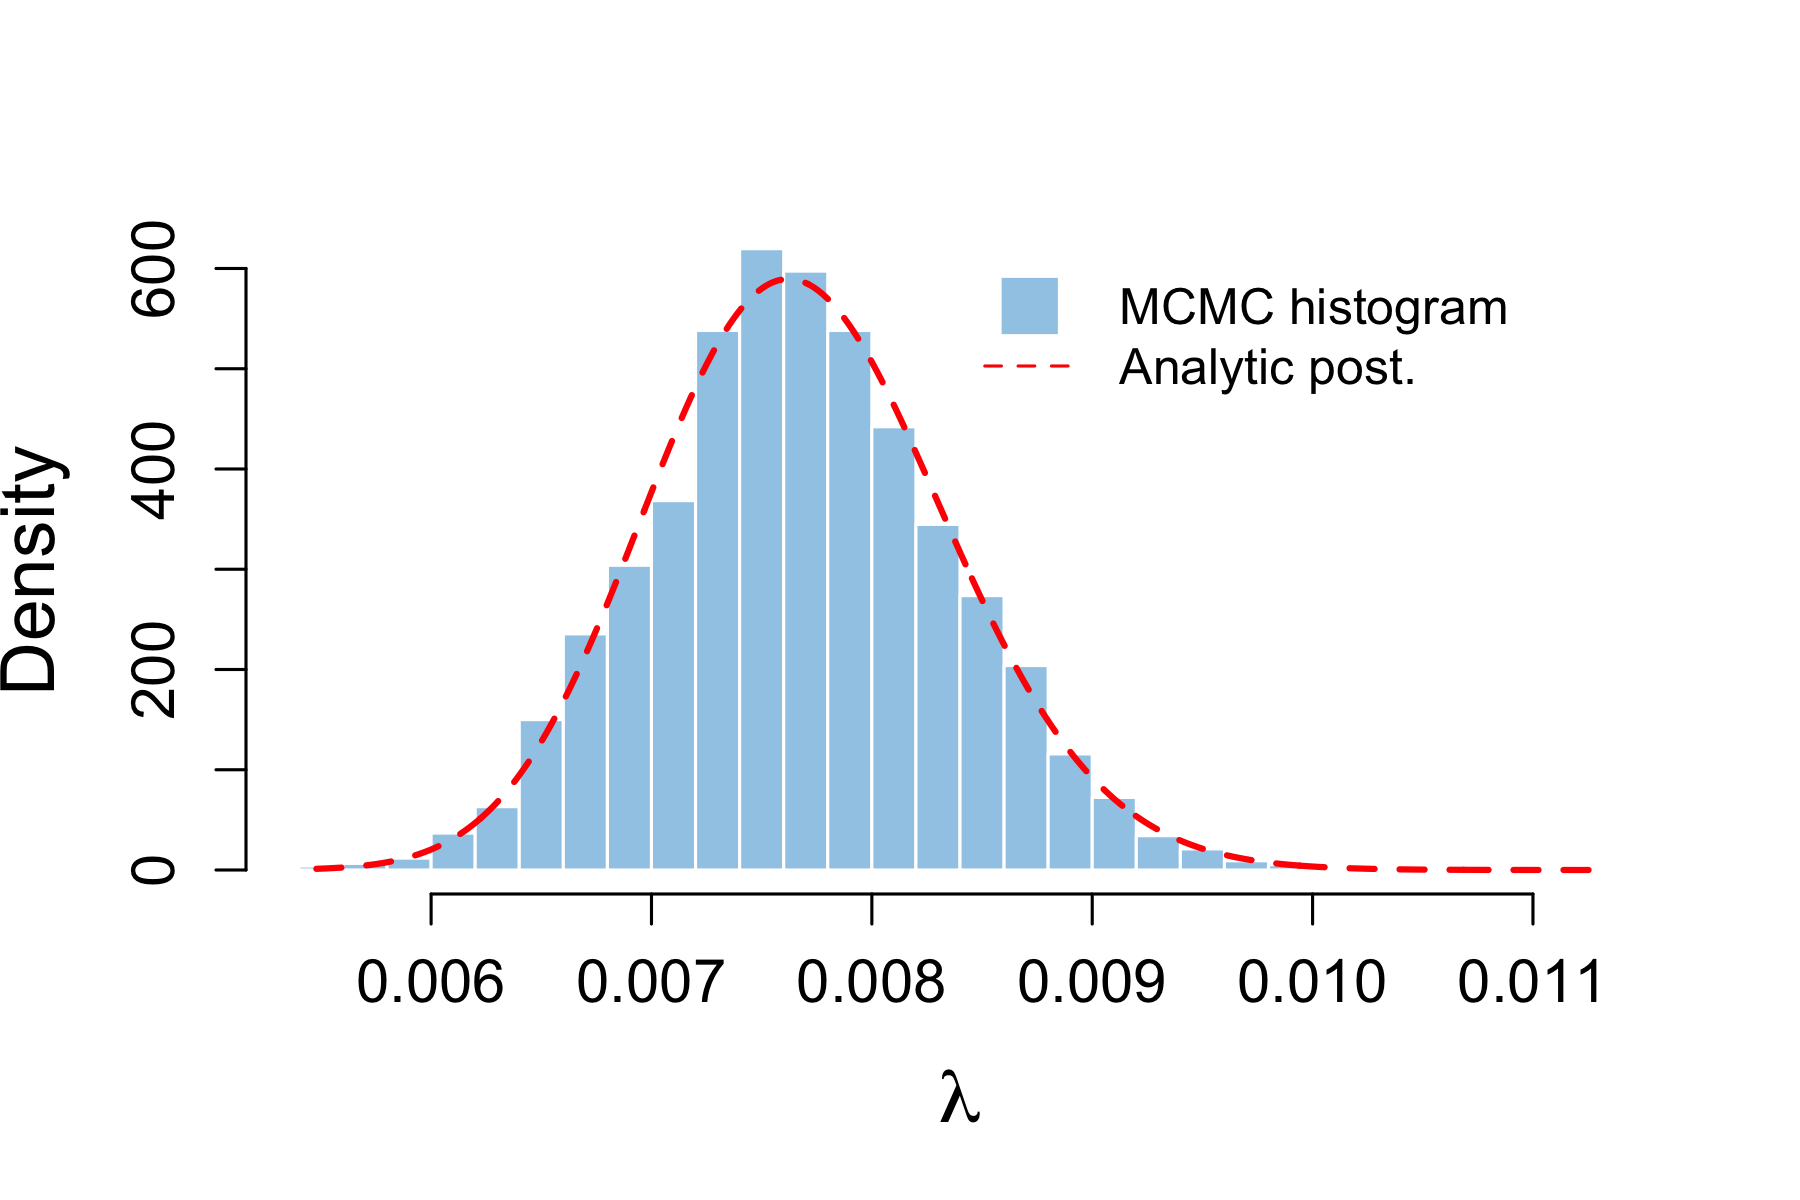
\includegraphics[height=8.5cm, width=0.59\textwidth]{images/veteran_post_lam.png}
    \caption{{\small Posterior distribution of $\lambda$ from MCMC samples (histogram) and analytic Gamma posterior (red curve) for the Veteran dataset.}}
    \label{fig:exp veteran}
\end{figure}





%%%%%%%%%%%%%%%%%%%%%%%%%%%%%%%%%%%%%%%%%%%%%%%%%%%%%%%%%%%%%%%%%%%%%%%%%%%%%%%%%%%%%%





\subsection{Model Checking}\label{sec:model checking}
\begin{figure}[H]
\centering
\resizebox{0.52\linewidth}{!}{
\begin{tikzpicture}[
 scale=0.50,
  every node/.style={transform shape}, 
  node distance=11mm,
  box/.style      ={rectangle, draw, rounded corners, align=center,
                    minimum width=44mm, minimum height=9mm},
  decision/.style ={diamond, aspect=2.2, draw, align=center, inner sep=1.4pt},
  ->, >=Latex
]

%--- Main process node ------------------------------------------------------
\node[box]      (model)   {\textbf{Define/Revise a model}};

\node[box]      (checking1)  [below=of model] {\textbf{Model checking} \\
(Simulate with $\lambda_0$; fit model; recover $\lambda_0$?)};

\node[decision] (pass1)   [below=10mm of checking1] {\textbf{Plausible?}};

\node[box]      (fit)     [below=of pass1]  {\textbf{Fit to real data}\\
(Compute posterior)};

\node[box]      (gen)     [below=of fit]    {\textbf{Posterior predictive model checking}\\
(Generate fake data from Posterior)\\
(Compare fake vs real)};

\node[decision] (pass2)   [below=of gen] {\textbf{Adequate?}};

\node[box]     (report)  [below=of pass2] {\textbf{Report/Interpret}};

%--- 连线 ------------------------------------------------------------
\draw (model)   -- (checking1)
      (checking1)  -- (pass1)
      (pass1)   -- node[right]{Yes}(fit)
      (fit)     -- (gen)
      (gen) -- (pass2)
      (pass2) -- node[right]{Yes}(report);

%--- Loopback ------------------------------------
\draw[->] (pass1.west) -- ++(-30mm,0) |- (model.west) node[pos=0.23, left]{No};
%\draw[->] (pass1.west) to[out=180,in=180,looseness=1.3] node[left]{No} (model.west);
\draw[->] (pass2.east) -- ++ (30mm,0 )|- (model.east) node[pos=0.23,right]{No};
\end{tikzpicture}}
\caption{General Bayesian workflow}
\end{figure}

\begin{tcolorbox}[
  title  = Algorithm 1: Simulating a Fake Survival Dataset (e.g.Posterior predictive model checking),
   fonttitle  = \small, 
  colback = white,
  colframe=black]
\textbf{Input}\\
\quad$\bullet$ posterior samples $\{\lambda^{(s)}\}$ \hfill (obtained by fitting real data)\\
\quad$\bullet$ sample size $n$ \hfill (same size as the real data set)\\
\quad$\bullet$ start‑time range $[a,0]$ with $a<0$ \\[6pt]
\textbf{Algorithm}\par
\begin{enumerate}
  \item Choose a single $\lambda^\ast$ from posterior samples \hfill (e.g.\ posterior mean)
  \item For $i = 1,\dots,n$
        \begin{enumerate}
          \item[] \hspace*{-10pt}%
          \begin{minipage}[t]{\linewidth}
          \begin{enumerate}
            \item Draw latent duration: $y_i \sim \operatorname{Exp}(\lambda^\ast)$
            \item Draw start time: $T_i \sim \operatorname{Uniform}(a,0)$
            \item Compute leaving time: $t_i = T_i + y_i$
            \item Observed pair $(\text{time}_i,\text{event}_i)$ \[\begin{aligned}
\text{if } \quad t_i &< 0: &&&\text{(event occurred before now)}\\
  &&\quad  \text{event}_i=1, &&\text{(uncensored)}\\ 
  &&\quad \text{time}_i=y_i
   &\quad \\
&\text{else}: &&&\text{(event in the future)}\\
   &&\quad \text{event}_i=0, &&\text{(right censored)}\\ 
   &&\quad \text{time}_i=-T_i &&\text{(time already spent)}
   &\quad 
\end{aligned}\]
          \end{enumerate}
          \end{minipage}
        \end{enumerate}
  \item Combine $(\text{time}_i,\text{event}_i)$ into a fake data set of size $n$.
\end{enumerate}
\label{fake data}
\end{tcolorbox}

\subsubsection{Model Checking via ECDF under Independent Censoring}
In model checking, to compare the overall distributional shapes of the real data and the simulated data, we use the empirical cumulative distribution function (ECDF) rather than histograms. Unlike histograms, ECDFs do not depend on subjective choices of bin widths and break points, thereby avoiding visual biases. Moreover, an ECDF is a monotone right-continuous step function defined on $[0,\infty)$, which stably displays differences between samples over the entire time axis. Importantly, ECDFs can be plugged directly into distance statistics such as the Kolmogorov–Smirnov or Cramér–von Mises metrics, facilitating quantitative assessment of model fit.

In survival data, the observed duration is determined jointly by the latent event time $T\ge 0$ and the censoring time $C\ge 0$. The observed quantity is
$$
Y=\min(T,C),\qquad \delta=\mathbf 1\{T\le C\}.
$$
That is, we observe the event time only when it is uncensored; otherwise, we observe the censoring time. Consequently, we split the data into two subsamples—an “event subsample’’ with $\delta=1$ and a “censored subsample’’ with $\delta=0$—and compute ECDFs for each subsample separately.

Under independent (non-informative) censoring, i.e., $T\perp C$, the two subsamples may be viewed as arising from two conditional distributions
\begin{itemize}
    \item for the event subsample ($\delta=1$), the observed values $Y=T$ follow the conditional distribution $T\mid(T\le C)$;
    \item for the censored subsample ($\delta=0$), the observed values $Y=C$ follow the conditional distribution $C\mid(C<T)$.
\end{itemize}
Let the event-subsample size be $n_1=\sum_i \delta_i$ and the censored-subsample size be $n_0=\sum_i (1-\delta_i)$. The corresponding empirical distribution functions are
\begin{equation}
    \widehat H_{\text{event}}(t)
=\frac{1}{n_1}\sum_{i:\,\delta_i=1}\mathbf 1\{Y_i\le t\},\qquad
\widehat H_{\text{cens}}(t)
=\frac{1}{n_0}\sum_{i:\,\delta_i=0}\mathbf 1\{Y_i\le t\},\qquad t\ge 0.
\end{equation}
By the Glivenko–Cantelli theorem (\cite{tucker1959generalization}), as sample sizes grow, these ECDFs converge uniformly to their respective target distribution functions
\begin{align}
\widehat H_{\text{event}}(t) &\xrightarrow{\text{uniformly in } t} H_{\text{event}}(t) := \Pr(T \le t \mid T \le C) \\
\widehat H_{\text{cens}}(t) &\xrightarrow{\text{uniformly in } t} H_{\text{cens}}(t) := \Pr(C \le t \mid C < T)
\end{align}
In summary, by splitting the data into event and censored subsamples and plotting their empirical distribution functions $\widehat H_{\text{event}}$ and $\widehat H_{\text{cens}}$, we can evaluate model fit within a unified framework along both dimensions.



%%%%%%%%%%%%%%%%%%%%%%%%%%%%%%%%%%%%%%%%%%%%%%%
\subsubsection{Choosing and Interpreting the Survey-Length Parameter $A$}

In the posterior predictive model checking of this study, we generate simulated data from the model and compare it with the observed data. This simulation relies on sampling given known quantities; a key quantity is the \textbf{maximum survey duration $A$ }in Algorithm 1 (\ref{fake data}), which is controlled by the user-specified parameter $a$, with the reparameterization $A = -a$, governing the censoring mechanism in the simulated data. In other words, $A$ sets the observation window in simulation and thereby affects both the censoring rate and the distribution of event times.

This quantity is not a parameter to be estimated by the model; it is an external input required to generate fake data. Although it may appear auxiliary, it is tightly coupled with model checking—different choices of $A$ change the censoring structure of the simulated data and therefore influence the credibility of posterior predictive results.

Does the observed data carry information about $A$? Yes. In any survival dataset, the “shadow” of the survey window is reflected in the censoring proportion and the shape of the observed durations. If the survey is short (small $A$), many subjects are censored before the event occurs, leading to a high right-censoring rate and “compressed” event times. Conversely, with a long survey (large $A$), more events are observed, censoring decreases, and event times spread out.

This can be seen in Figure~\ref{fig:离职数据分开的直方图} (histograms of event and censored durations in the employee turnover data). The number of events and censors is roughly balanced, suggesting that the survey was long enough to capture about half of the departures. Since the maximum observed duration exceeds 170 months, it is reasonable to infer that the underlying survey duration $A$ should be at least greater than 170; this directly informs how the censoring mechanism should be set in simulation.
\begin{figure}[H]
    \centering
    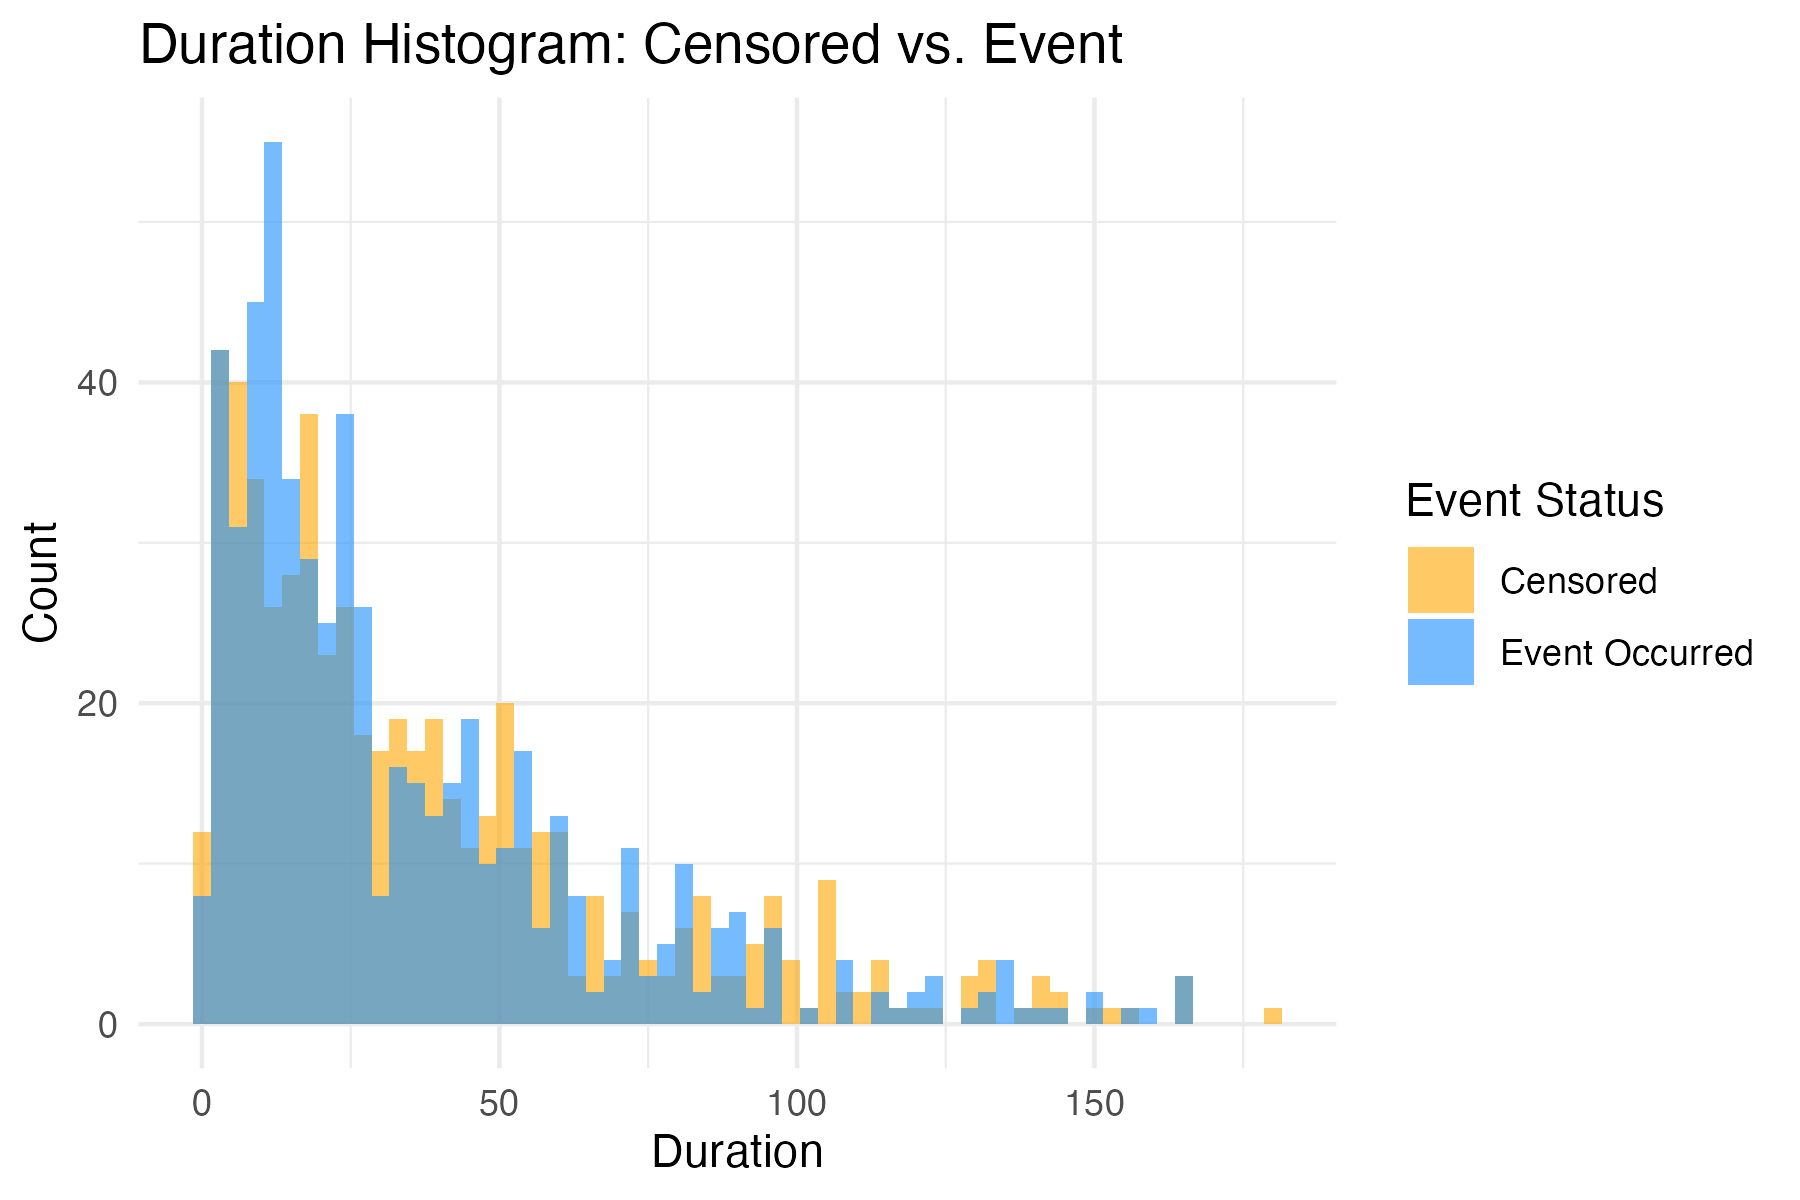
\includegraphics[height=5.5cm, width=0.6\textwidth]{images/separate_hist.png}
    \caption{Histograms of censored and event durations in the employee turnover data}
    \label{fig:离职数据分开的直方图}
\end{figure}
To further support this point, we simulate under two settings, $A = 30$ and $A = 1000$, and plot the empirical cumulative distribution functions (ECDFs) for both the event subsample ($\delta = 1$) and the censored subsample ($\delta = 0$), along with the histograms of simulated durations.
\begin{itemize}
    \item $A = 30$ (Figure~\ref{fig:ppc-A30}). Compared to the real-data histogram (Figure~\ref{fig:离职数据分开的直方图}), the simulated durations in Figure~\ref{fig:fake-hist_a30} are heavily compressed within 0–30 months, indicating that both events and censorings occur unusually early. Correspondingly, the ECDFs for events and censorings (Figure~\ref{fig:ecdf-cens_a30}~\ref{fig:ecdf-event_a30}, red lines) rise too steeply at short durations, deviating noticeably from the observed curves. This mismatch is primarily driven by an unrealistic observation window $A$, rather than a misfit of the event-time distribution (e.g., the parameter $\lambda$) itself.
    \item $A = 1000$ (Figure~\ref{fig:ppc-A1000})
  In contrast, Figure~\ref{fig:fake-hist_a1000} shows a histogram with a much wider and sparser spread of durations, and the ECDF curves (Figure~\ref{fig:ecdf-event_a1000}~\ref{fig:ecdf-cens_a1000}, red lines) align more closely with the observed data. However, when compared to the real-data histogram in Figure~\ref{fig:离职数据分开的直方图}, this setting exceeds any realistic survey length—implying a maximum tenure close to 83 years—which is implausible in practical employment contexts. Thus, although the simulated curves fit better visually, this apparent “match” relies on an unrealistic assumption about $A$, and should not be accepted as a reliable model-checking result.
\end{itemize}
These two examples reinforce a key point: when performing posterior predictive checks, fit quality must be evaluated alongside the realism of the data-generating assumptions in simulation.
\begin{figure}[htbp]
\centering
\begin{subfigure}[t]{0.3\textwidth}
  \centering
  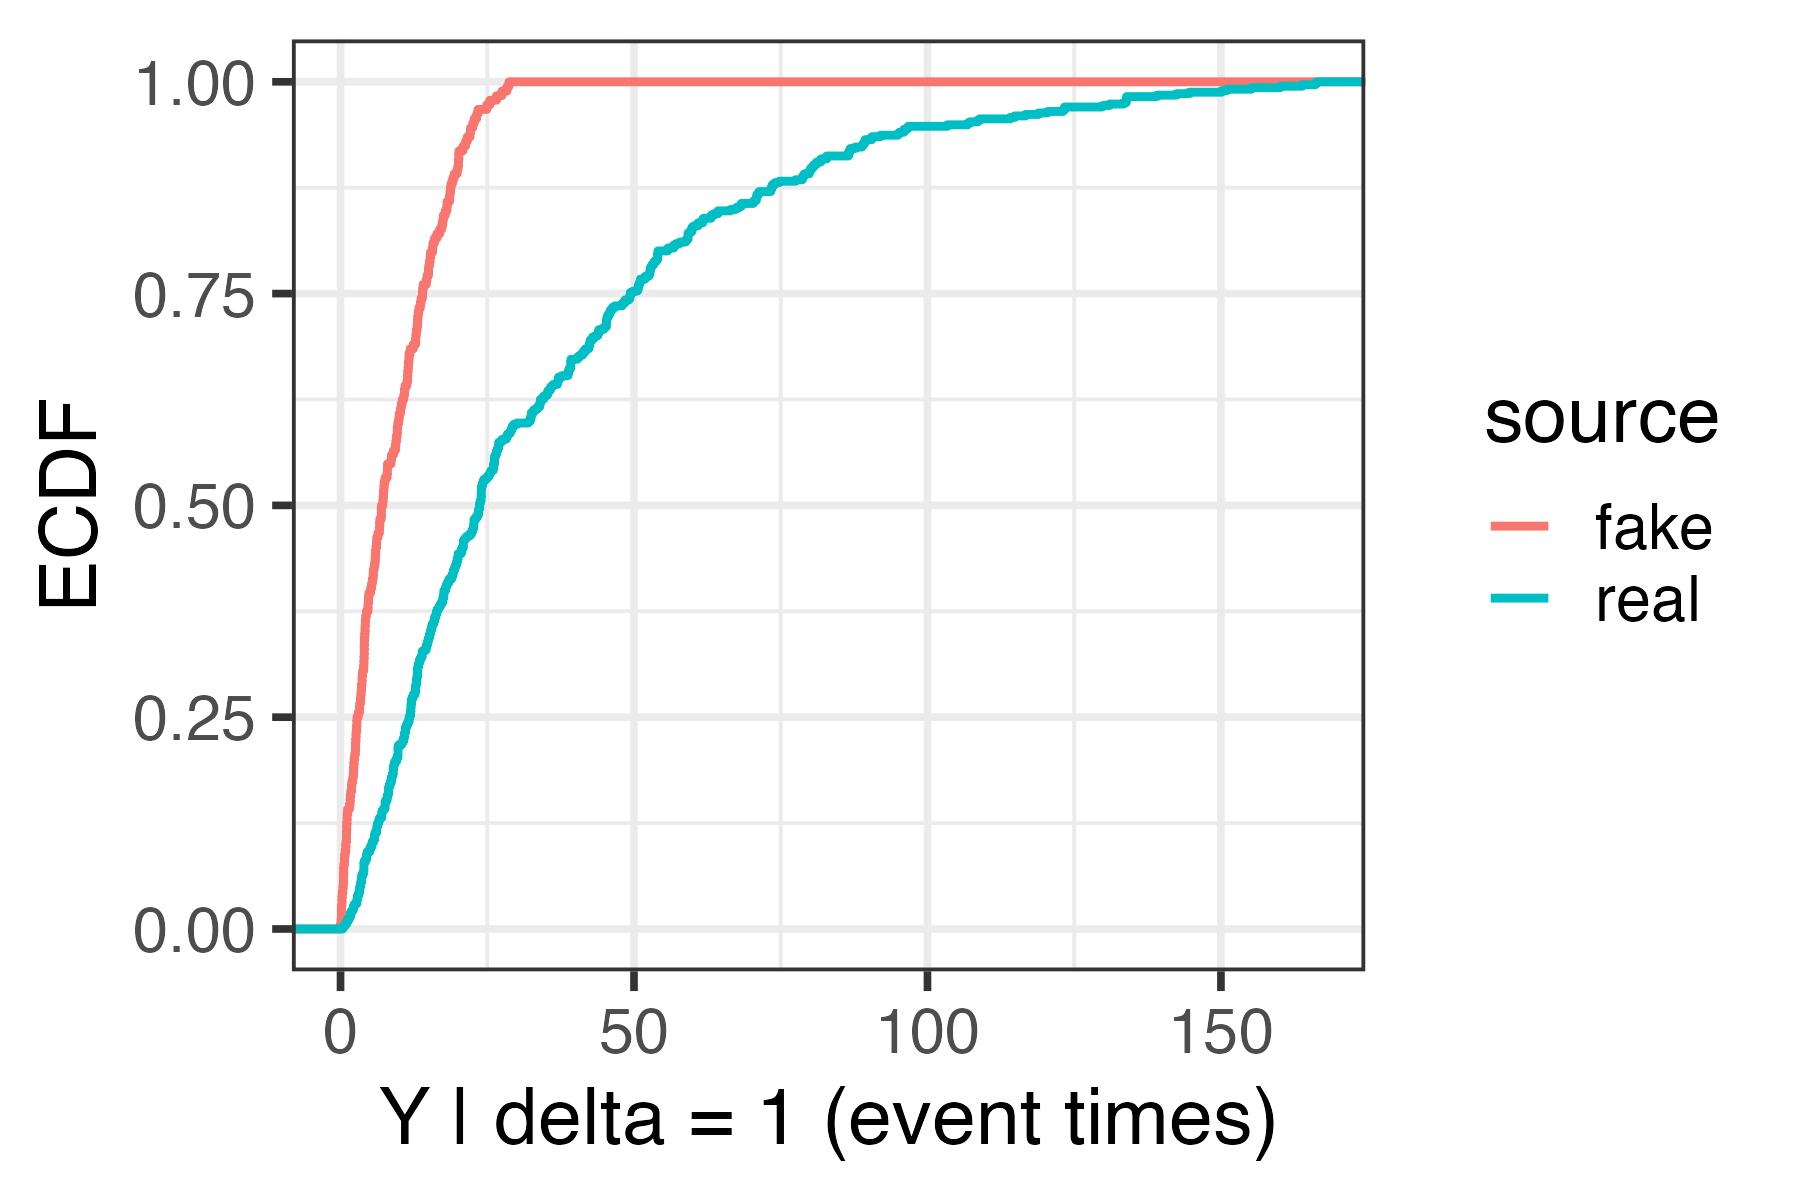
\includegraphics[width=\linewidth]{images/ppc_event_ecdf_A30.png}  % 图1路径
  \caption{ECDF of $Y \mid \delta=1$}
  \label{fig:ecdf-event_a30}
\end{subfigure}\hfill
\begin{subfigure}[t]{0.3\textwidth}
  \centering
  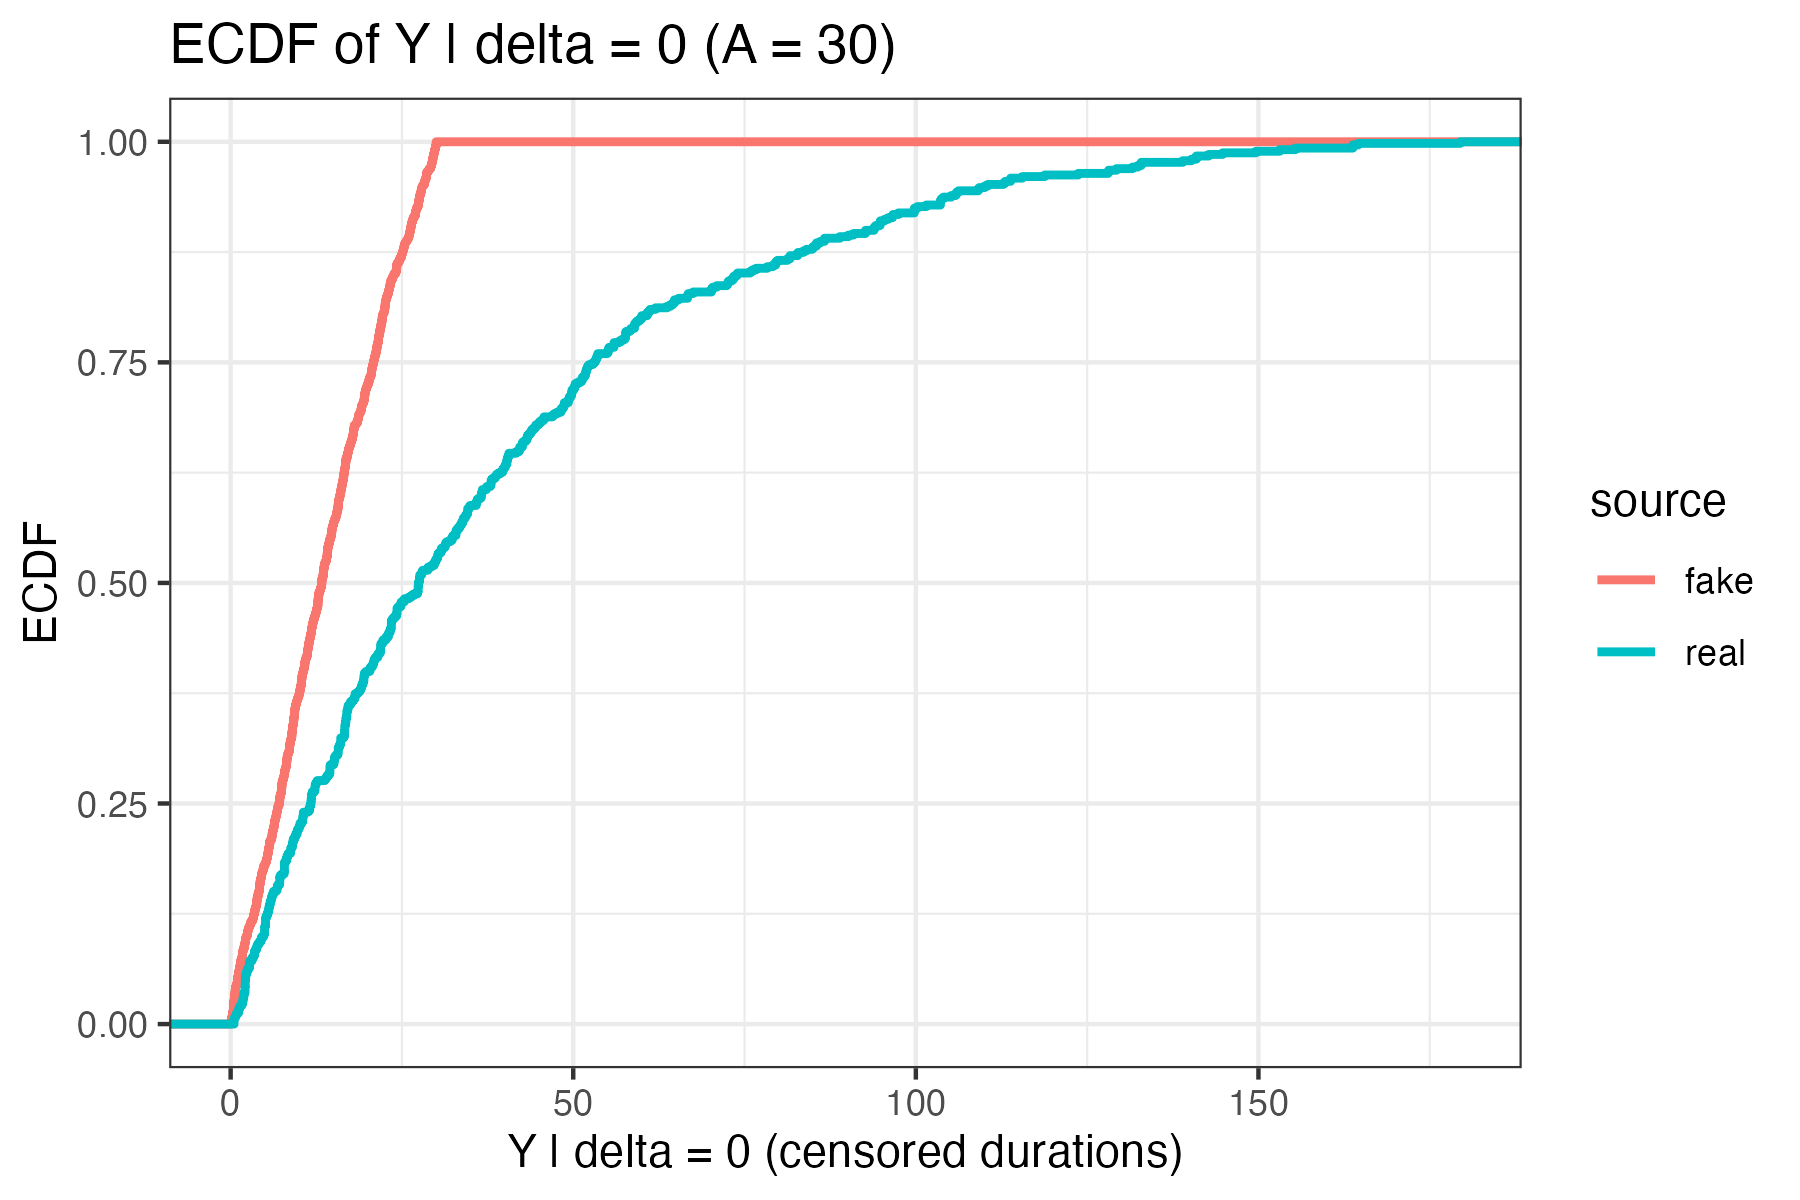
\includegraphics[width=\linewidth]{images/ppc_censored_ecdf_A30.png}   
  \caption{ECDF of $Y \mid \delta=0$}
  \label{fig:ecdf-cens_a30}
\end{subfigure}\hfill
\begin{subfigure}[t]{0.37\textwidth}
  \centering
  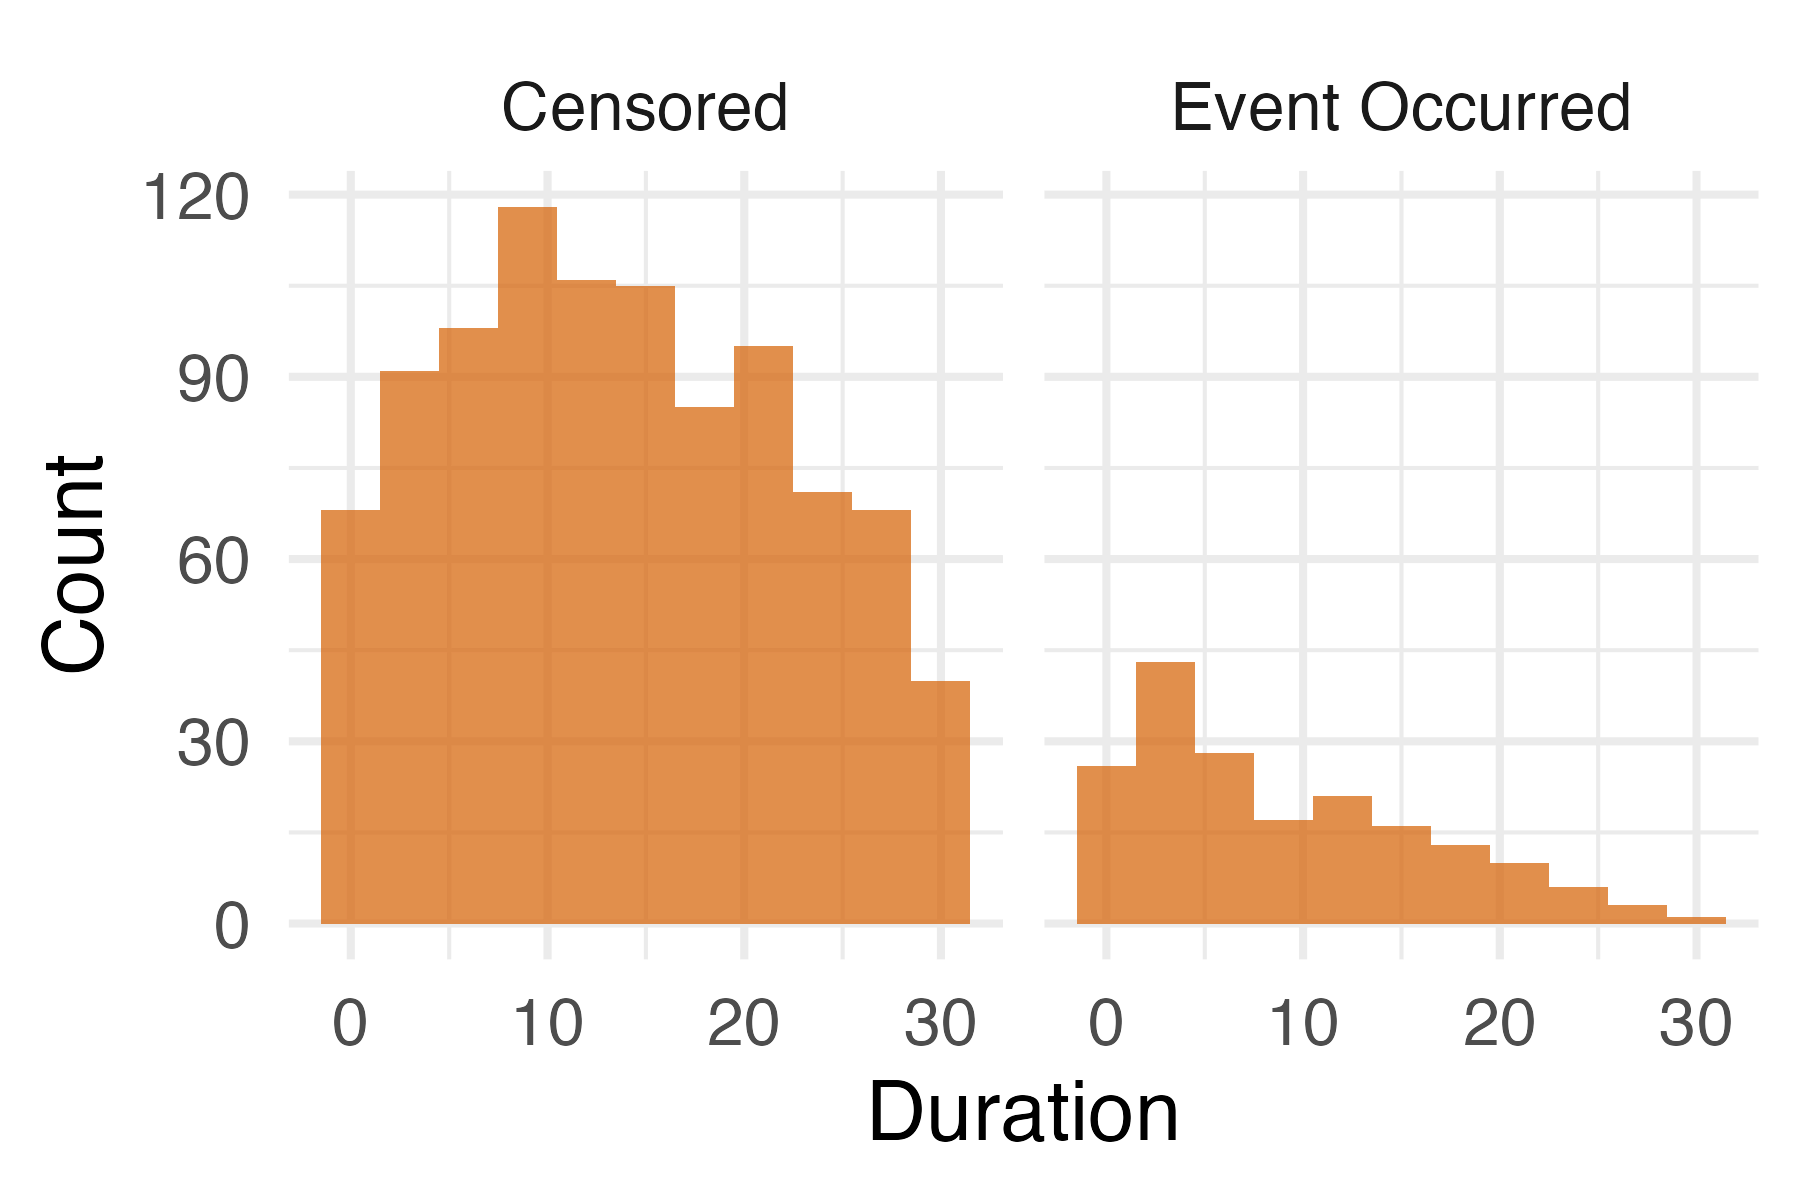
\includegraphics[width=\linewidth]{images/fake_duration_hist_a30.png}   % 图3路径
  \caption{Fake-data histogram}
  \label{fig:fake-hist_a30}
\end{subfigure}
\caption{Posterior predictive checking ($A=30$).}
\label{fig:ppc-A30}
\end{figure}
%%%%%%%%%%%%%%%%%%%%%%
\begin{figure}[htbp]
\centering
\begin{subfigure}[t]{0.3\textwidth}
  \centering
  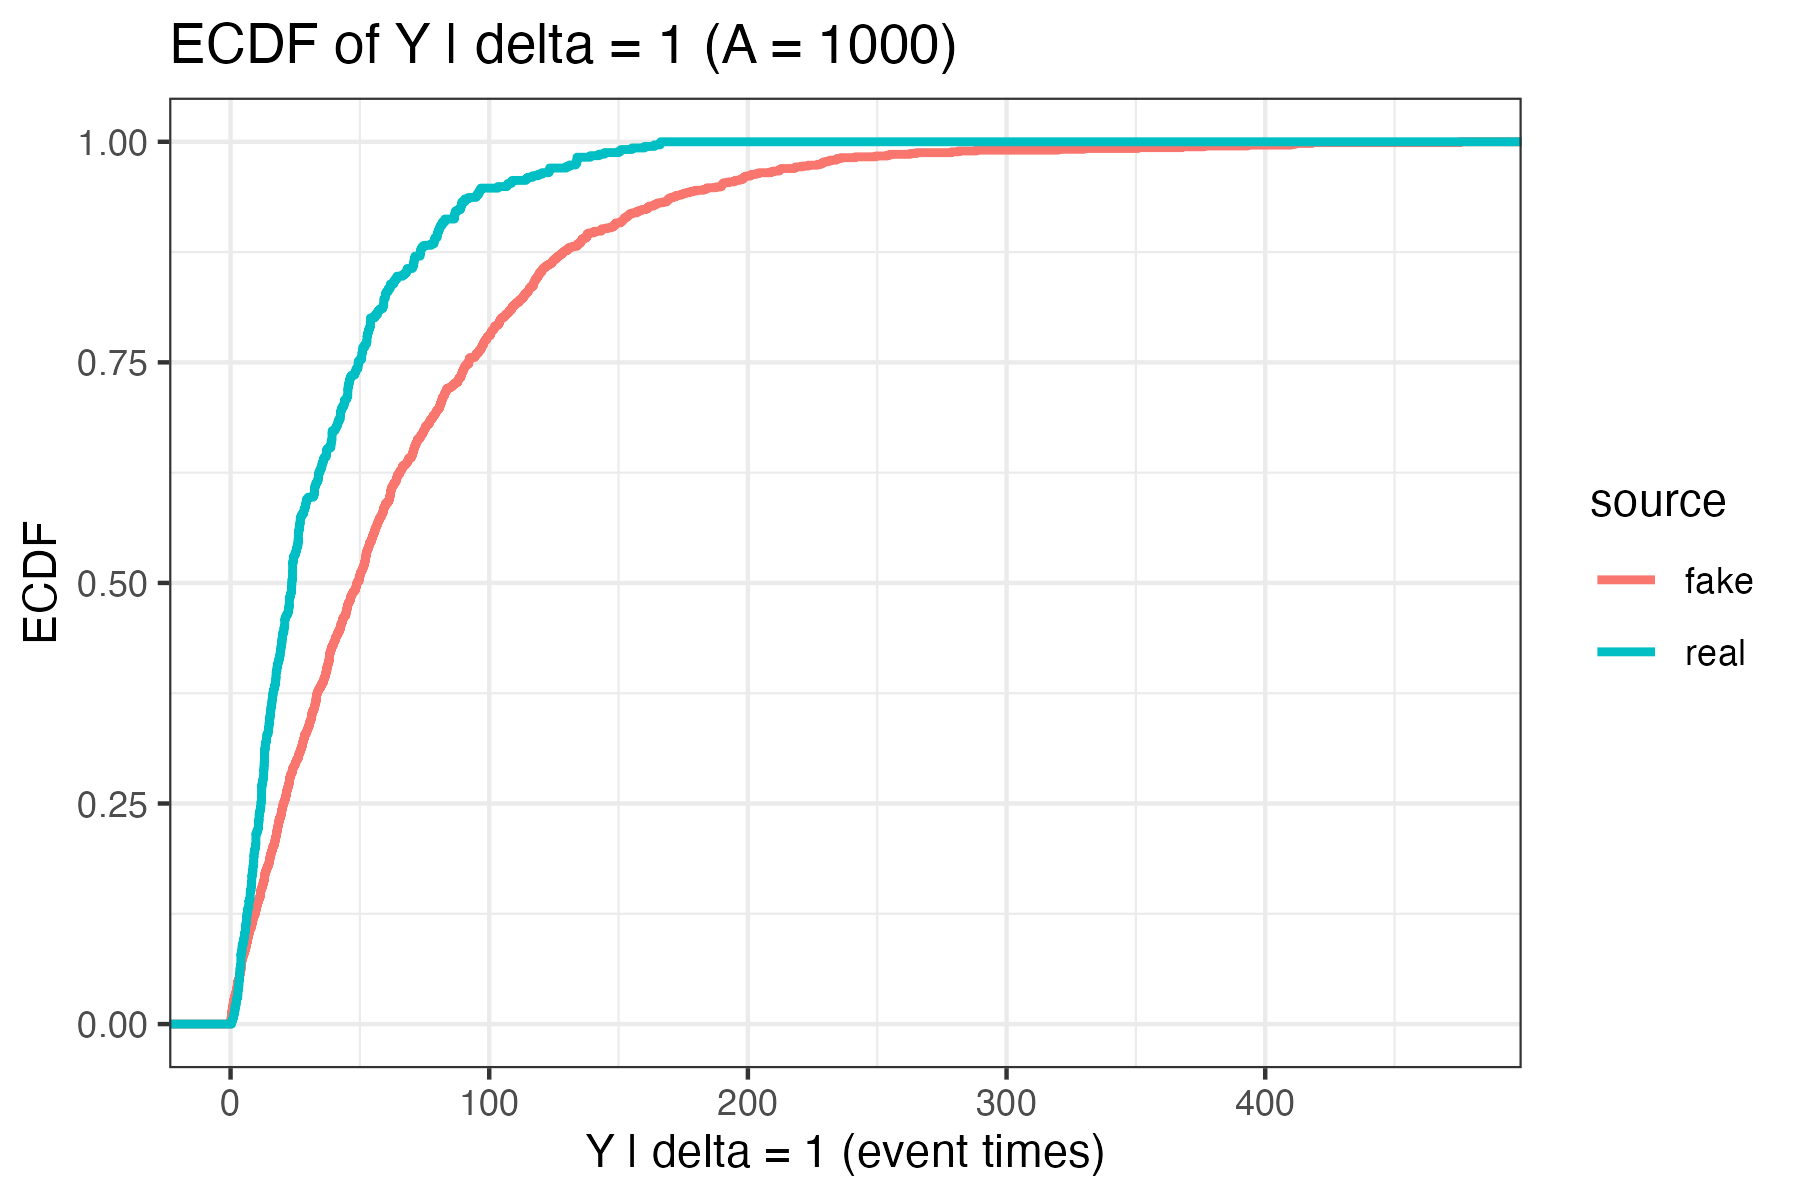
\includegraphics[width=\linewidth]{images/ppc_event_ecdf_A1000.png}  % 图1路径
  \caption{ECDF of $Y \mid \delta=1$}
  \label{fig:ecdf-event_a1000}
\end{subfigure}\hfill
\begin{subfigure}[t]{0.3\textwidth}
  \centering
  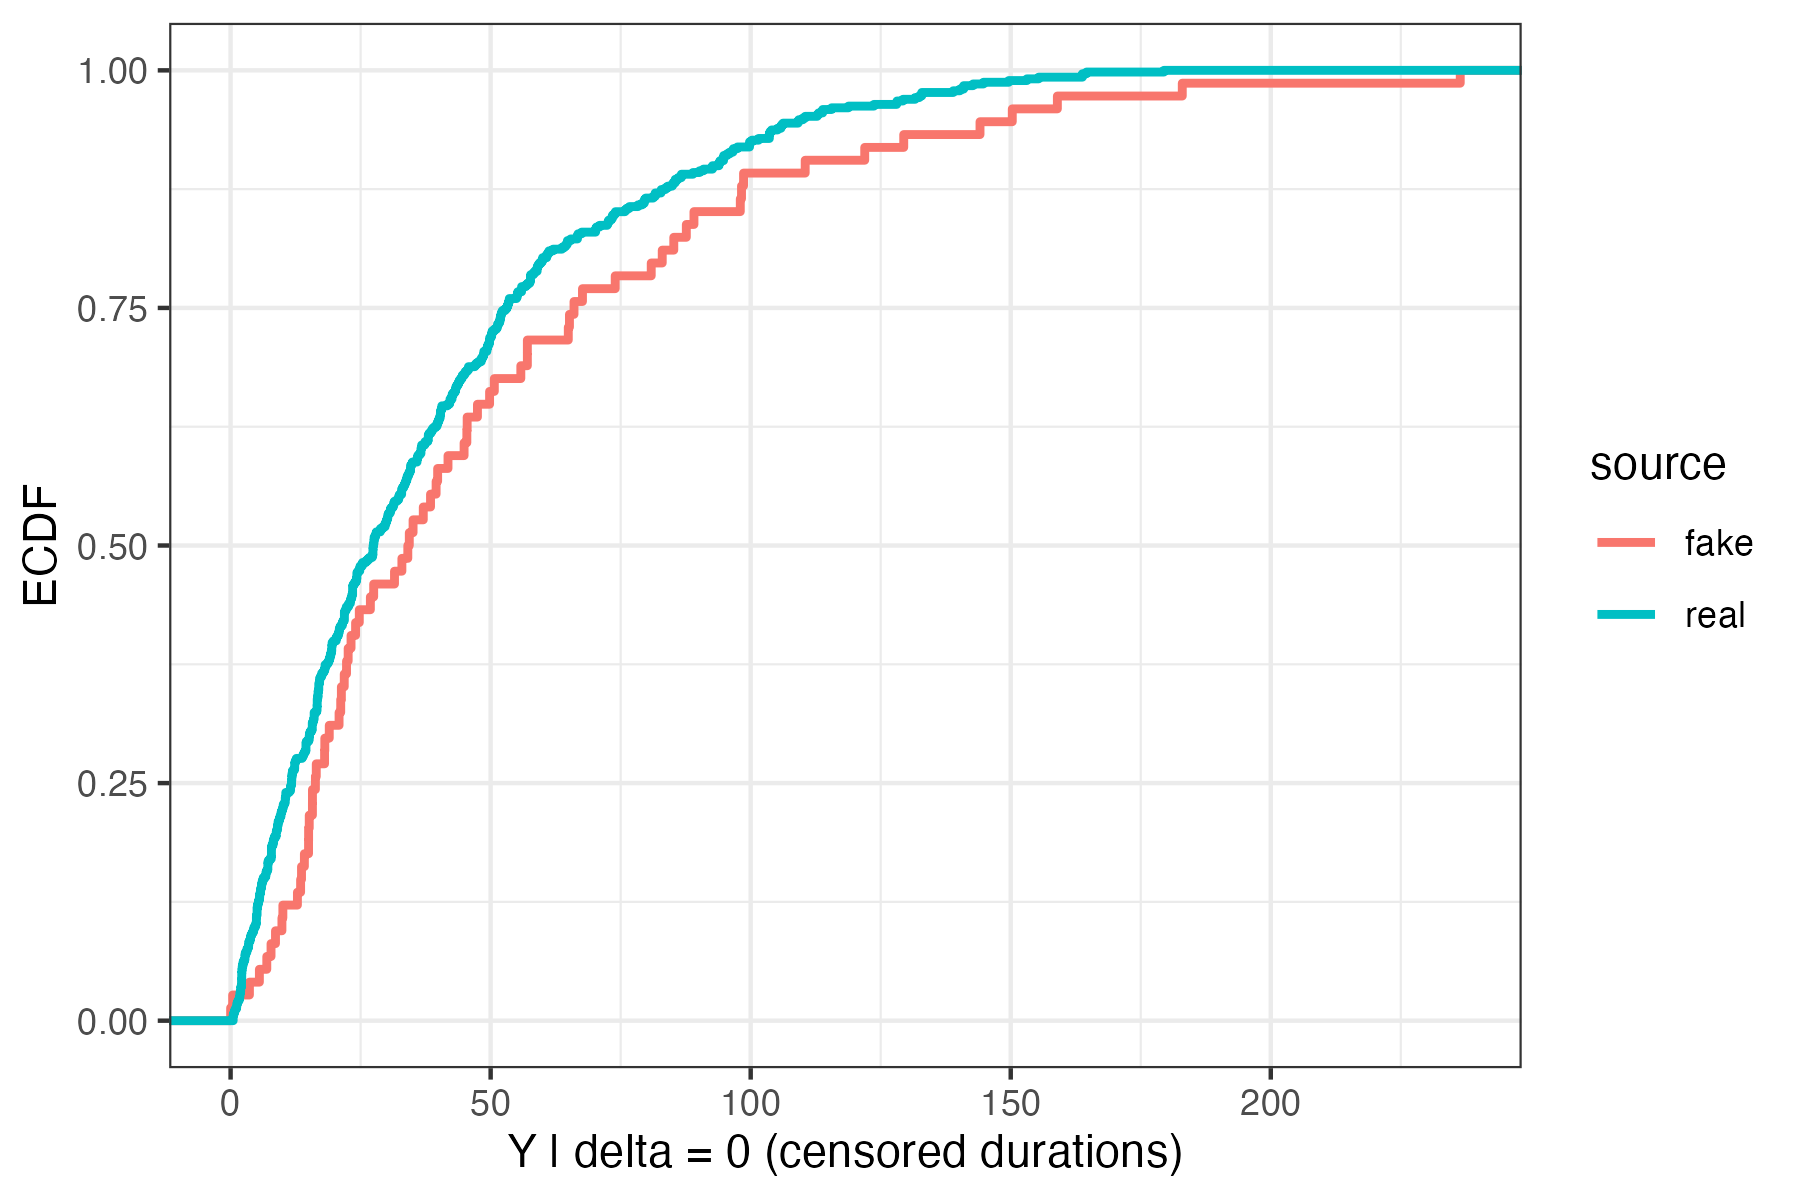
\includegraphics[width=\linewidth]{images/ppc_censored_ecdf_A1000.png} 
  \caption{ECDF of $Y \mid \delta=0$}
  \label{fig:ecdf-cens_a1000}
\end{subfigure}\hfill
\begin{subfigure}[t]{0.37\textwidth}
  \centering
  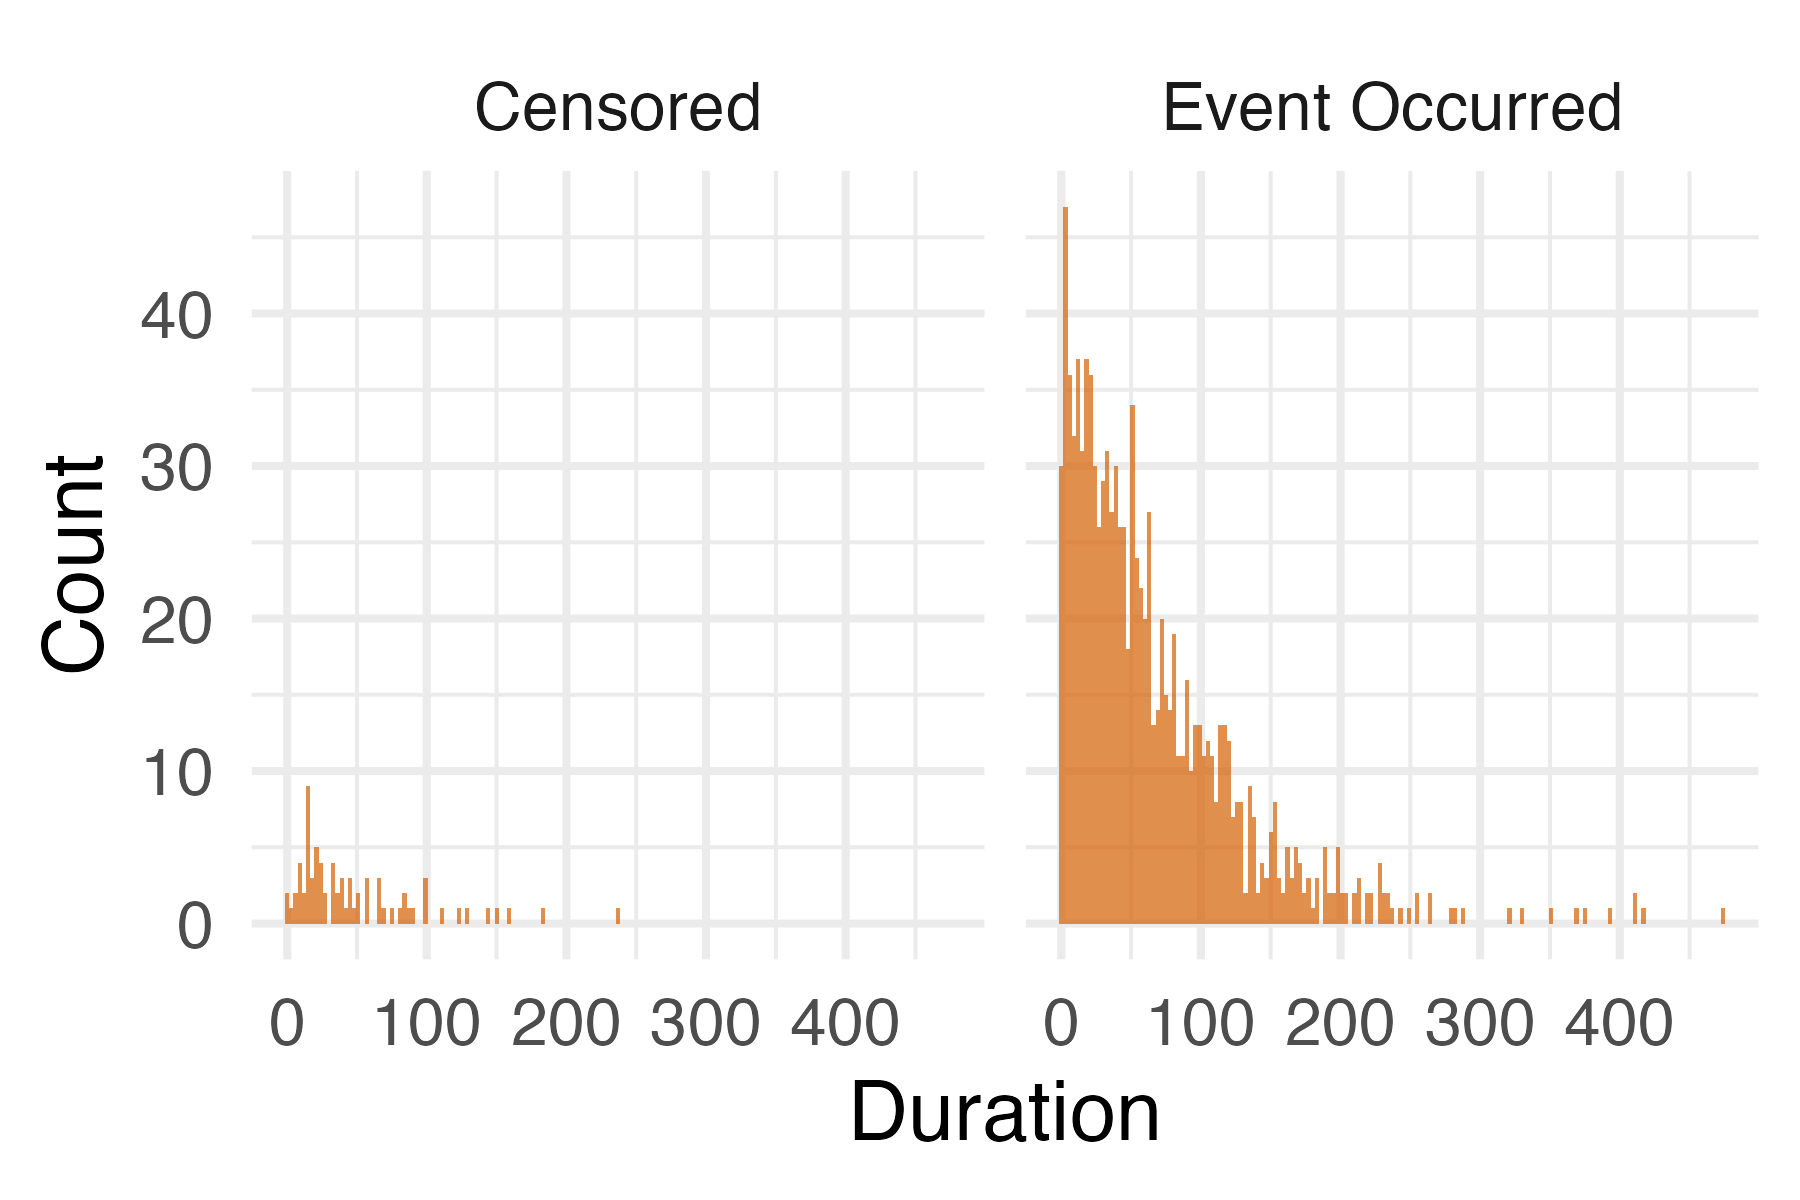
\includegraphics[width=\linewidth]{images/fake_duration_hist_a1000.png}   % 图3路径
  \caption{Fake-data histogram}
  \label{fig:fake-hist_a1000}
\end{subfigure}
\caption{Posterior predictive checking ($A=1000$).}
\label{fig:ppc-A1000}
\end{figure}


%\subsection{Posterior predictive CDF}
%\input{MSc_Statistics_Research_Report_paper/section/Methods_subsection/posterior predictive cdf }






\subsection{Impact of the Survey-Length Parameter \texorpdfstring{$A$}{A} on Censoring and Model Fit}
\label{Impact of A}
In the posterior predictive model checking of this study (Section~\ref{subsec:wo Layers of Model Checking}), we found that the \textbf{maximum survey duration $A$}, controlling the censoring mechanism in Algorithm 1 through the reparameterization $A$, has a substantial influence on simulation outcomes and the credibility of posterior predictive results. In simulation, $A$ defines the observation window, thereby determining both the censoring rate and the distribution of event times. Although $A$ is not estimated by the baseline model, it is a key external setting when generating fake data. Different choices of $A$ alter the censoring structure and can change the conclusions drawn from posterior predictive checks, making $A$ tightly coupled with model checking.

Does the observed data carry information about $A$? Yes. In any survival dataset, the “shadow” of the survey window is reflected in the censoring proportion and the shape of the observed durations. If $A$ is small, many subjects are censored before the event occurs, leading to a high right-censoring rate and “compressed” event times. Conversely, a large $A$ yields more observed events, lower censoring, and more dispersed event times.

Figure~\ref{fig:离职数据分开的直方图} separates event and censored durations in the employee turnover data. The roughly balanced counts suggest the survey captured about half of the departures. Since the maximum observed duration exceeds 170 months, $A$ should be at least above this threshold. While this alone does not pinpoint $A$, exploratory simulations show that around 200 months yields censoring patterns most consistent with the observed data. This insight guides realistic simulation design and helps to rule out implausibly small (e.g., $A=30$) or excessively large (e.g., $A=1000$) settings. In a Bayesian framework, when $A$ is included in the likelihood, such information will be reflected in its posterior distribution—this is the focus of the next section.
\begin{figure}[H]
    \centering
    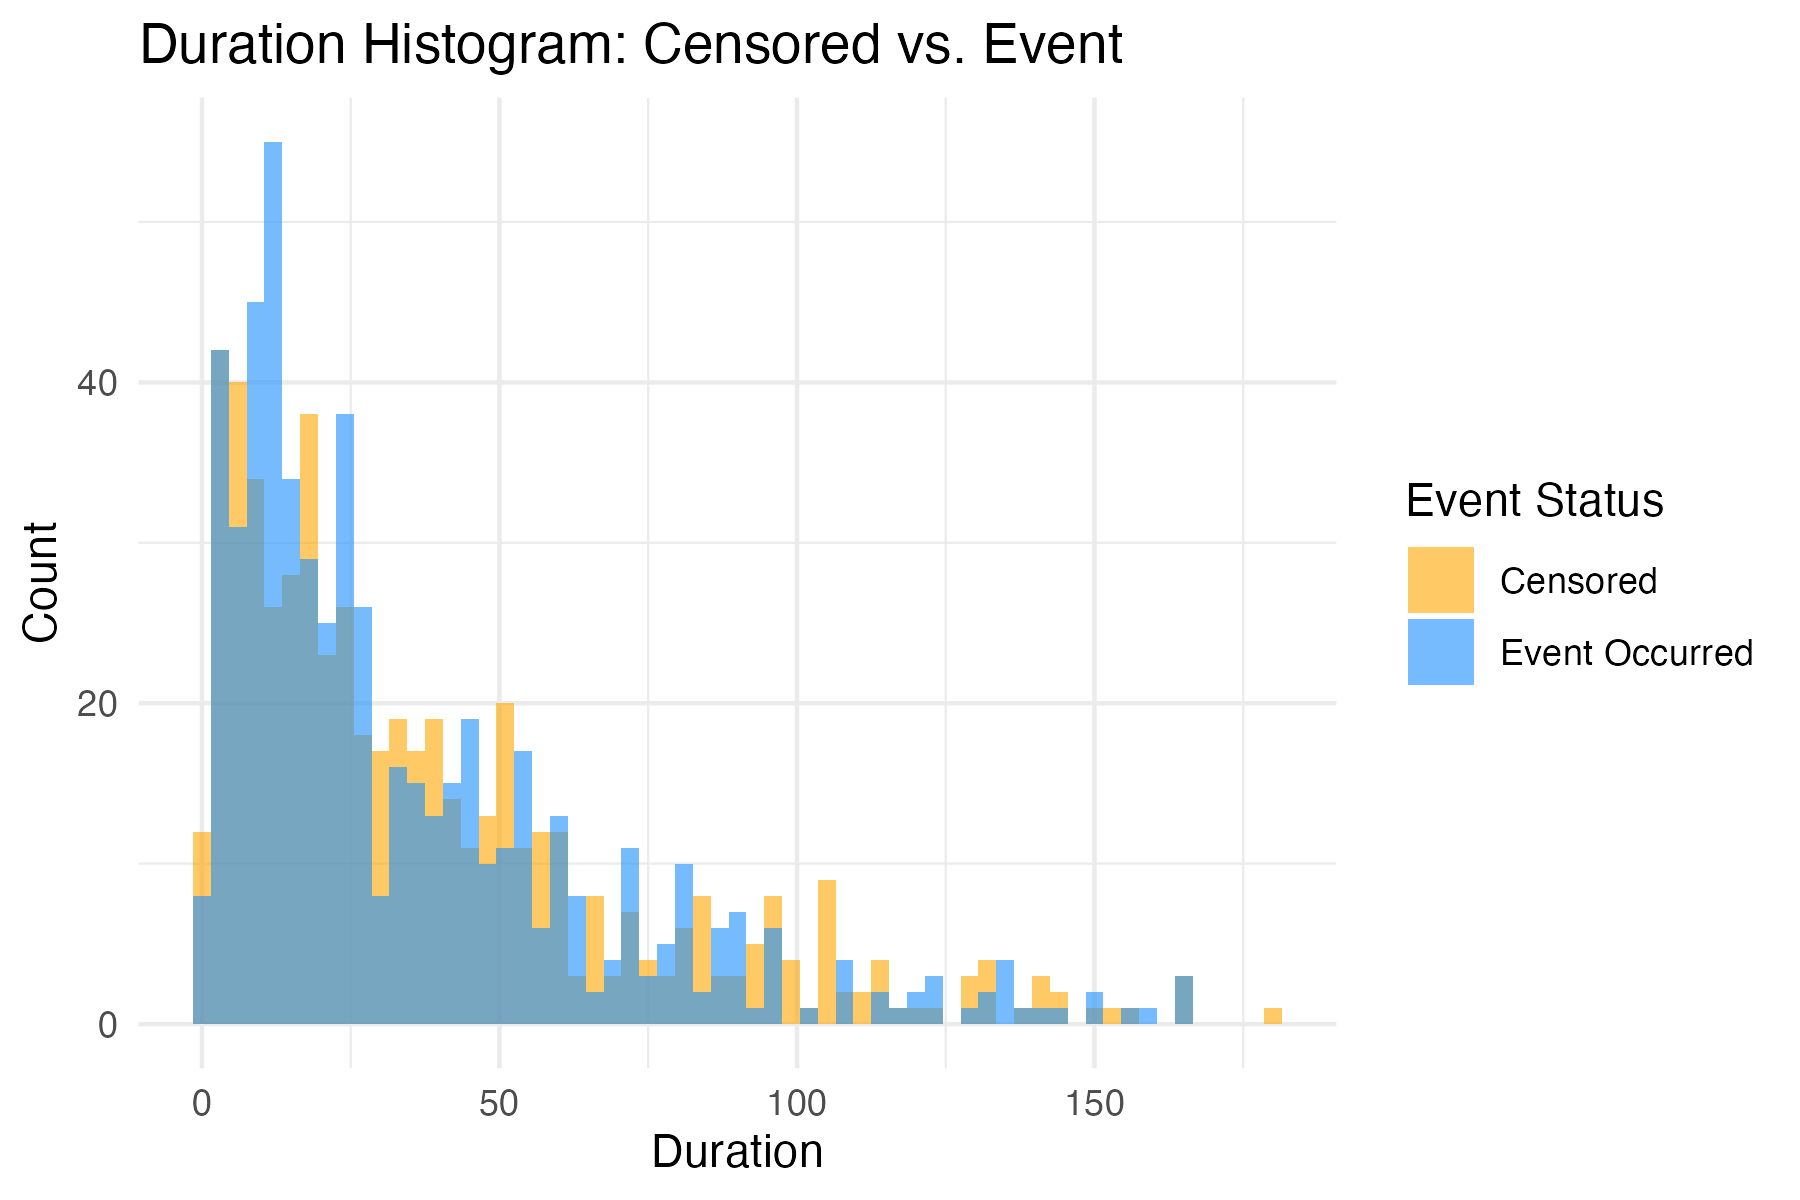
\includegraphics[height=5.5cm, width=0.6\textwidth]{images/separate_hist.png}
    \caption{{\small Histograms of censored and event durations in the employee turnover data}}
    \label{fig:离职数据分开的直方图}
\end{figure}
To illustrate the effect of unrealistic observation windows, we simulate under two settings, $A = 30$ and $A = 1000$, and plot the empirical cumulative distribution functions (ECDFs) for both the event subsample ($\delta = 1$) and the censored subsample ($\delta = 0$), along with the histograms of simulated durations.
\begin{itemize}
    \item $A = 30$ (Figure~\ref{fig:ppc-A30}). Relative to the real-data histogram (Figure~\ref{fig:离职数据分开的直方图}), simulated durations are tightly compressed within 0–30 months, with both events and censorings occurring unusually early. The ECDFs (Figure~\ref{fig:ecdf-event_a30}–\ref{fig:ecdf-cens_a30}, red lines) rise sharply at short durations and diverge from the observed curves, highlighting the impact of an unrealistically small $A$ rather than any misfit in the event-time parameter $\lambda$.
    \item $A = 1000$ (Figure~\ref{fig:ppc-A1000}). The simulated histogram in Figure~\ref{fig:fake-hist_a1000} shows durations that are widely dispersed, and the ECDF curves (Figure~\ref{fig:ecdf-event_a1000}–\ref{fig:ecdf-cens_a1000}, red lines) align more closely with the observed data than in the $A=30$ case. However, when compared with the real-data histogram in Figure~\ref{fig:离职数据分开的直方图}, this setting implies a maximum tenure approaching 83 years—far beyond any realistic employment scenario. The apparent visual agreement is therefore driven by an implausible survey window rather than by an accurate recovery of the event-time distribution, making such a setting unsuitable for credible model checking.
\end{itemize}
\begin{figure}[H]
\centering
\begin{subfigure}[t]{0.32\textwidth}
  \centering
  \includegraphics[width=\textwidth]{images/}  % 图1路径
  \caption{{\small ECDF of $Y \mid \delta=1$}}
  \label{fig:ecdf-event_a30}
\end{subfigure}
%\begin{subfigure}[t]{0.32\textwidth}
  %\centering
  %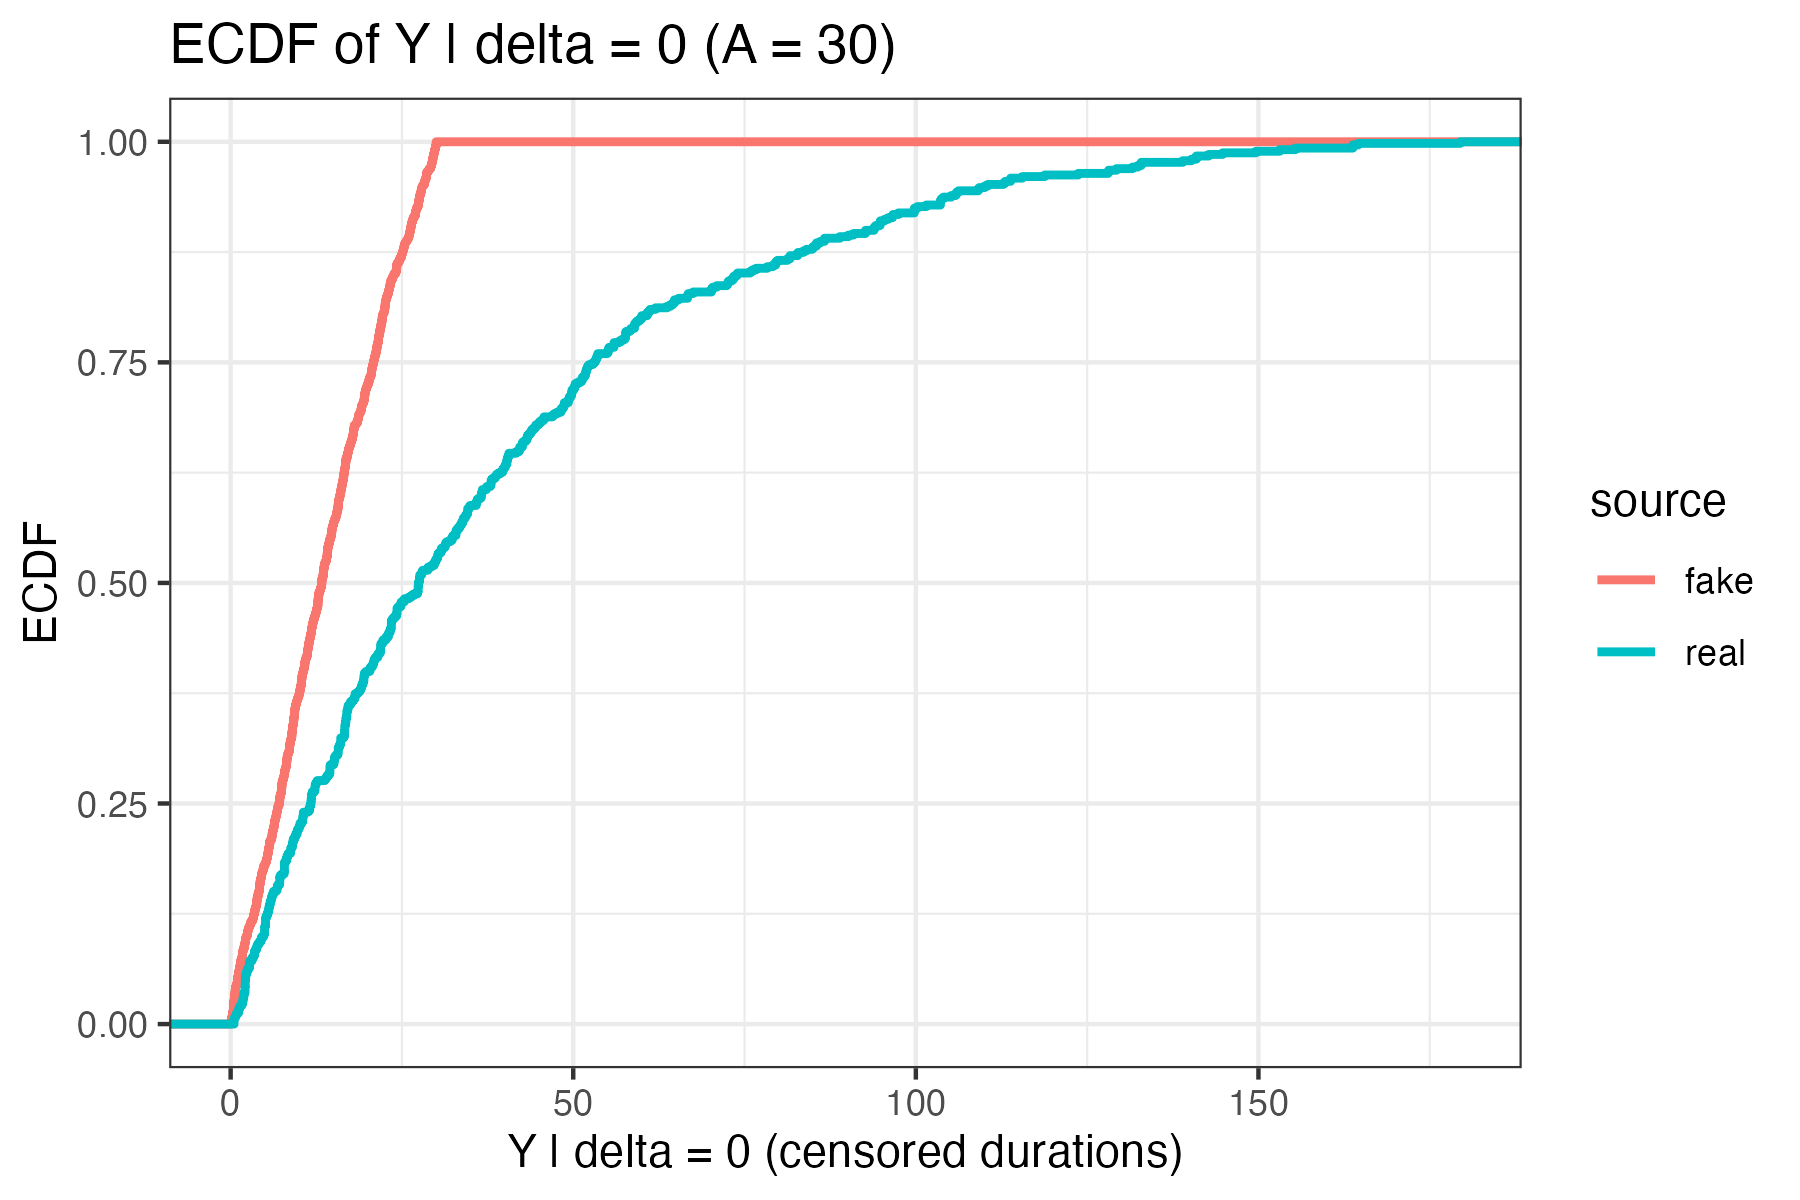
\includegraphics[width=\linewidth]{images/ppc_censored_ecdf_A30.png}   
  %\caption{{\small ECDF of $Y \mid \delta=0$}}
  %\end{subfigure}\hfill
\begin{subfigure}[t]{0.35\textwidth}
  \centering
  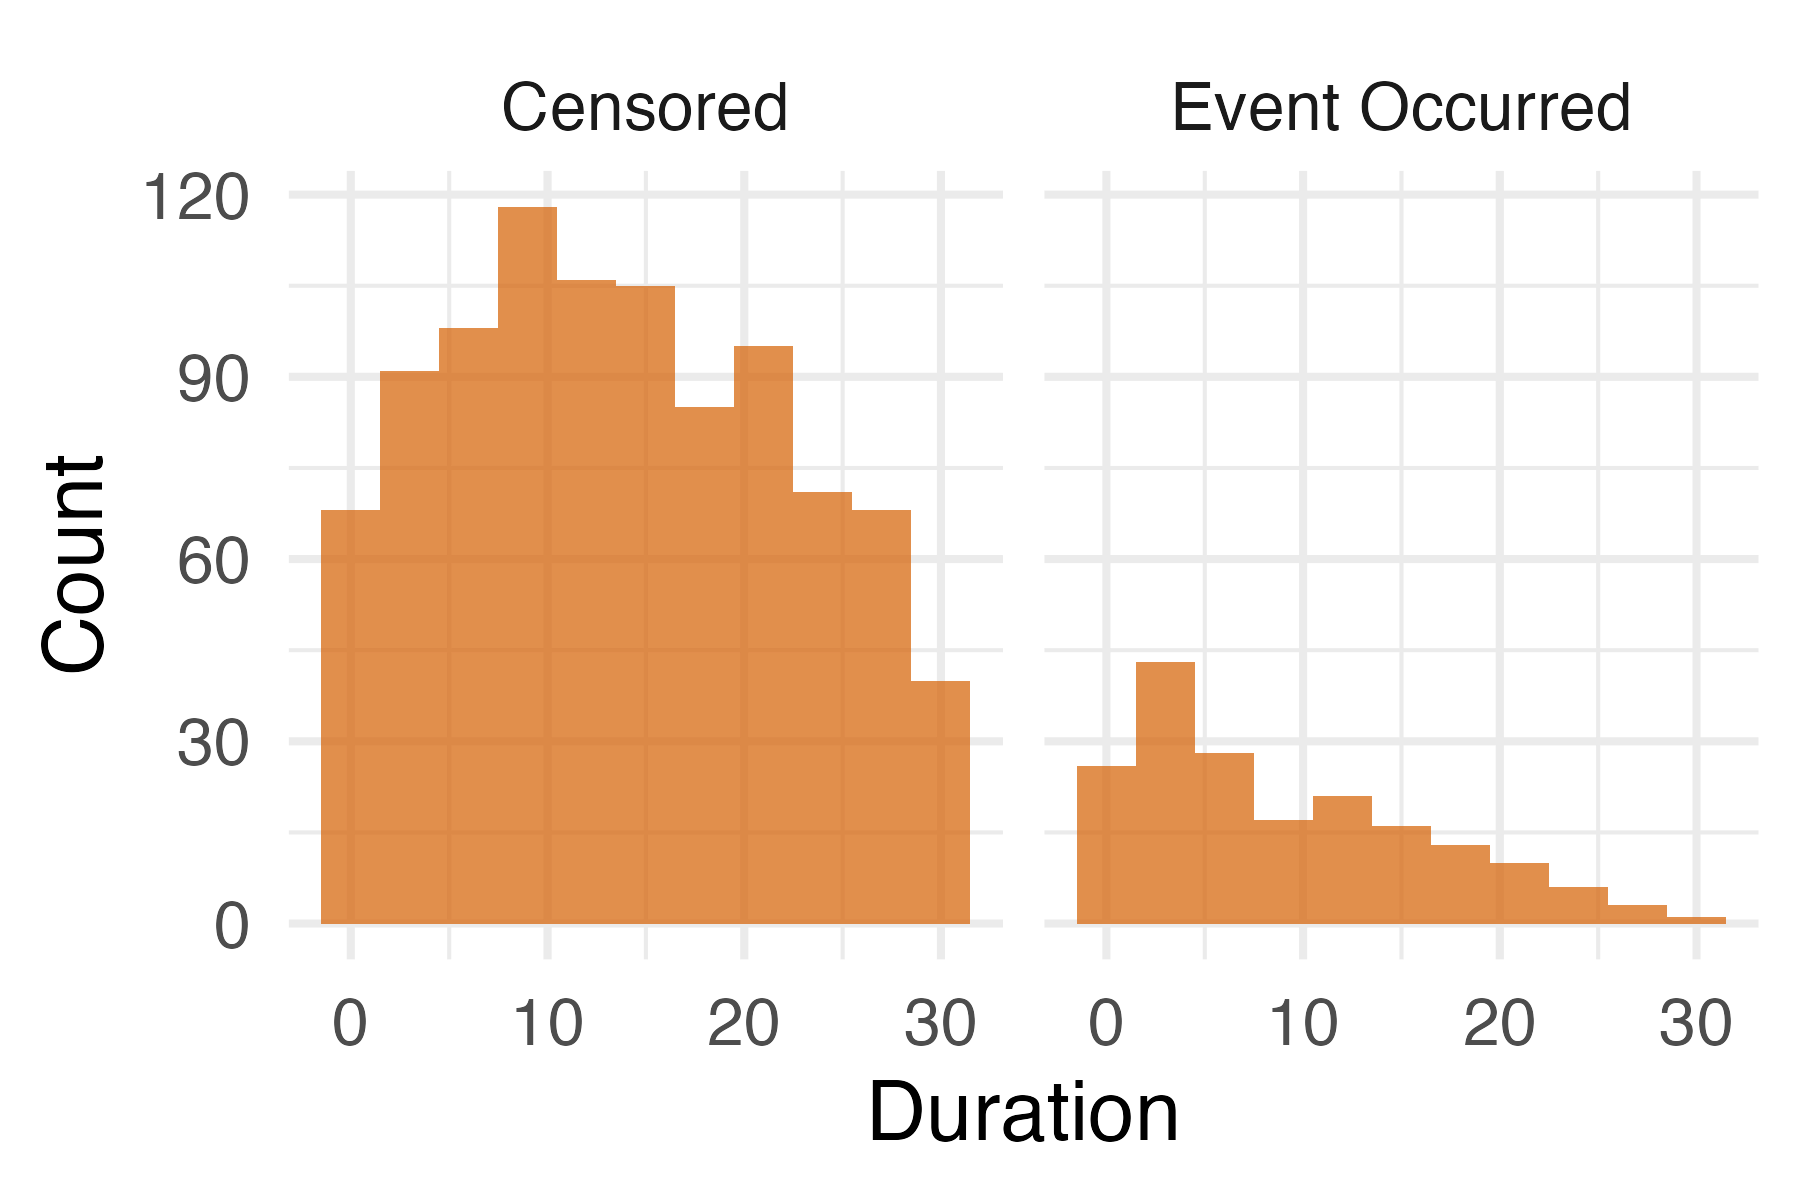
\includegraphics[width=\linewidth]{images/fake_duration_hist_a30.png}   % 图3路径
  \caption{{\small Fake-data histogram}}
  \label{fig:fake-hist_a30}
\end{subfigure}
\caption{{\small Posterior predictive checking ($A=30$).}}
\label{fig:ppc-A30}
\end{figure}
%%%%%%%%%%%%%%%%%%%%%%
\begin{figure}[H]
\centering
\begin{subfigure}[t]{0.3\textwidth}
  \centering
  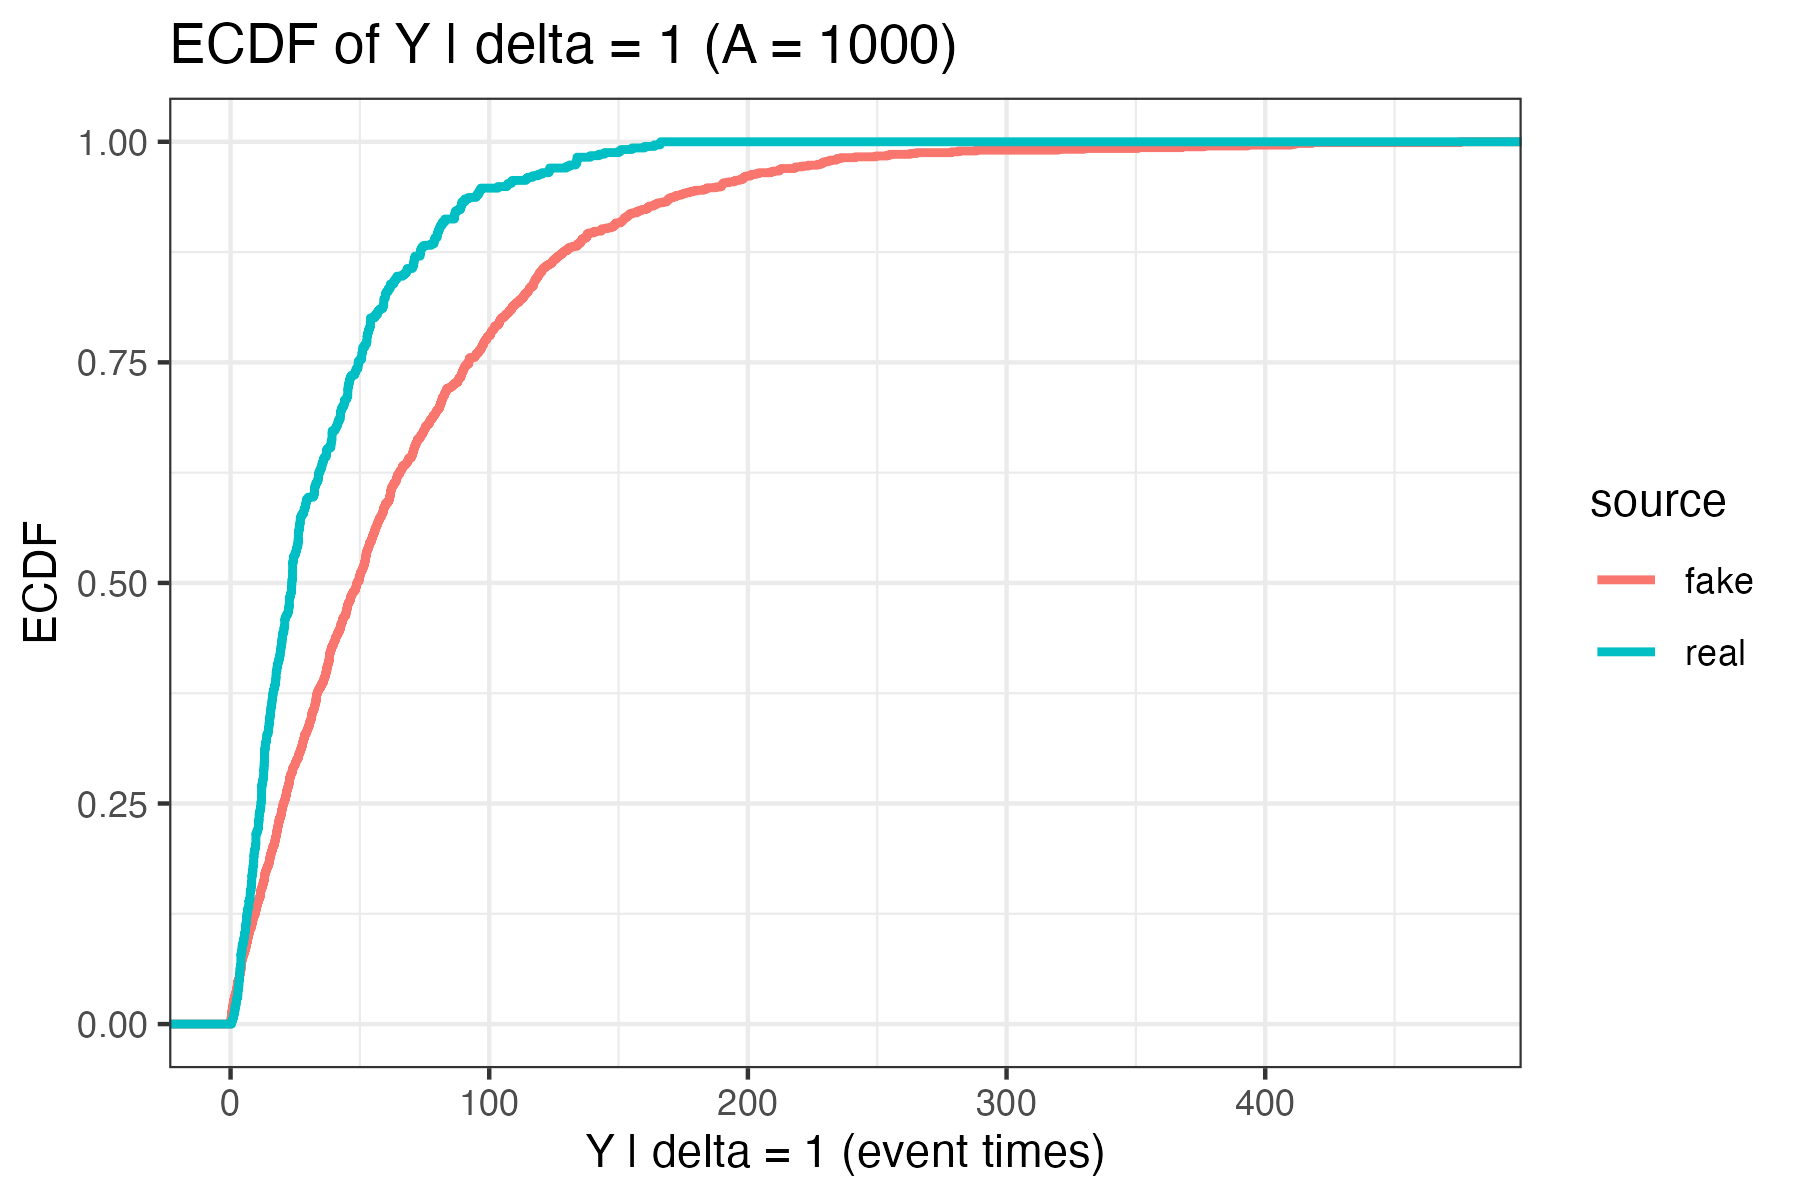
\includegraphics[width=\linewidth]{images/ppc_event_ecdf_A1000.png}  % 图1路径
  \caption{{\small ECDF of $Y \mid \delta=1$}}
  \label{fig:ecdf-event_a1000}
\end{subfigure}\hfill
\begin{subfigure}[t]{0.3\textwidth}
  \centering
  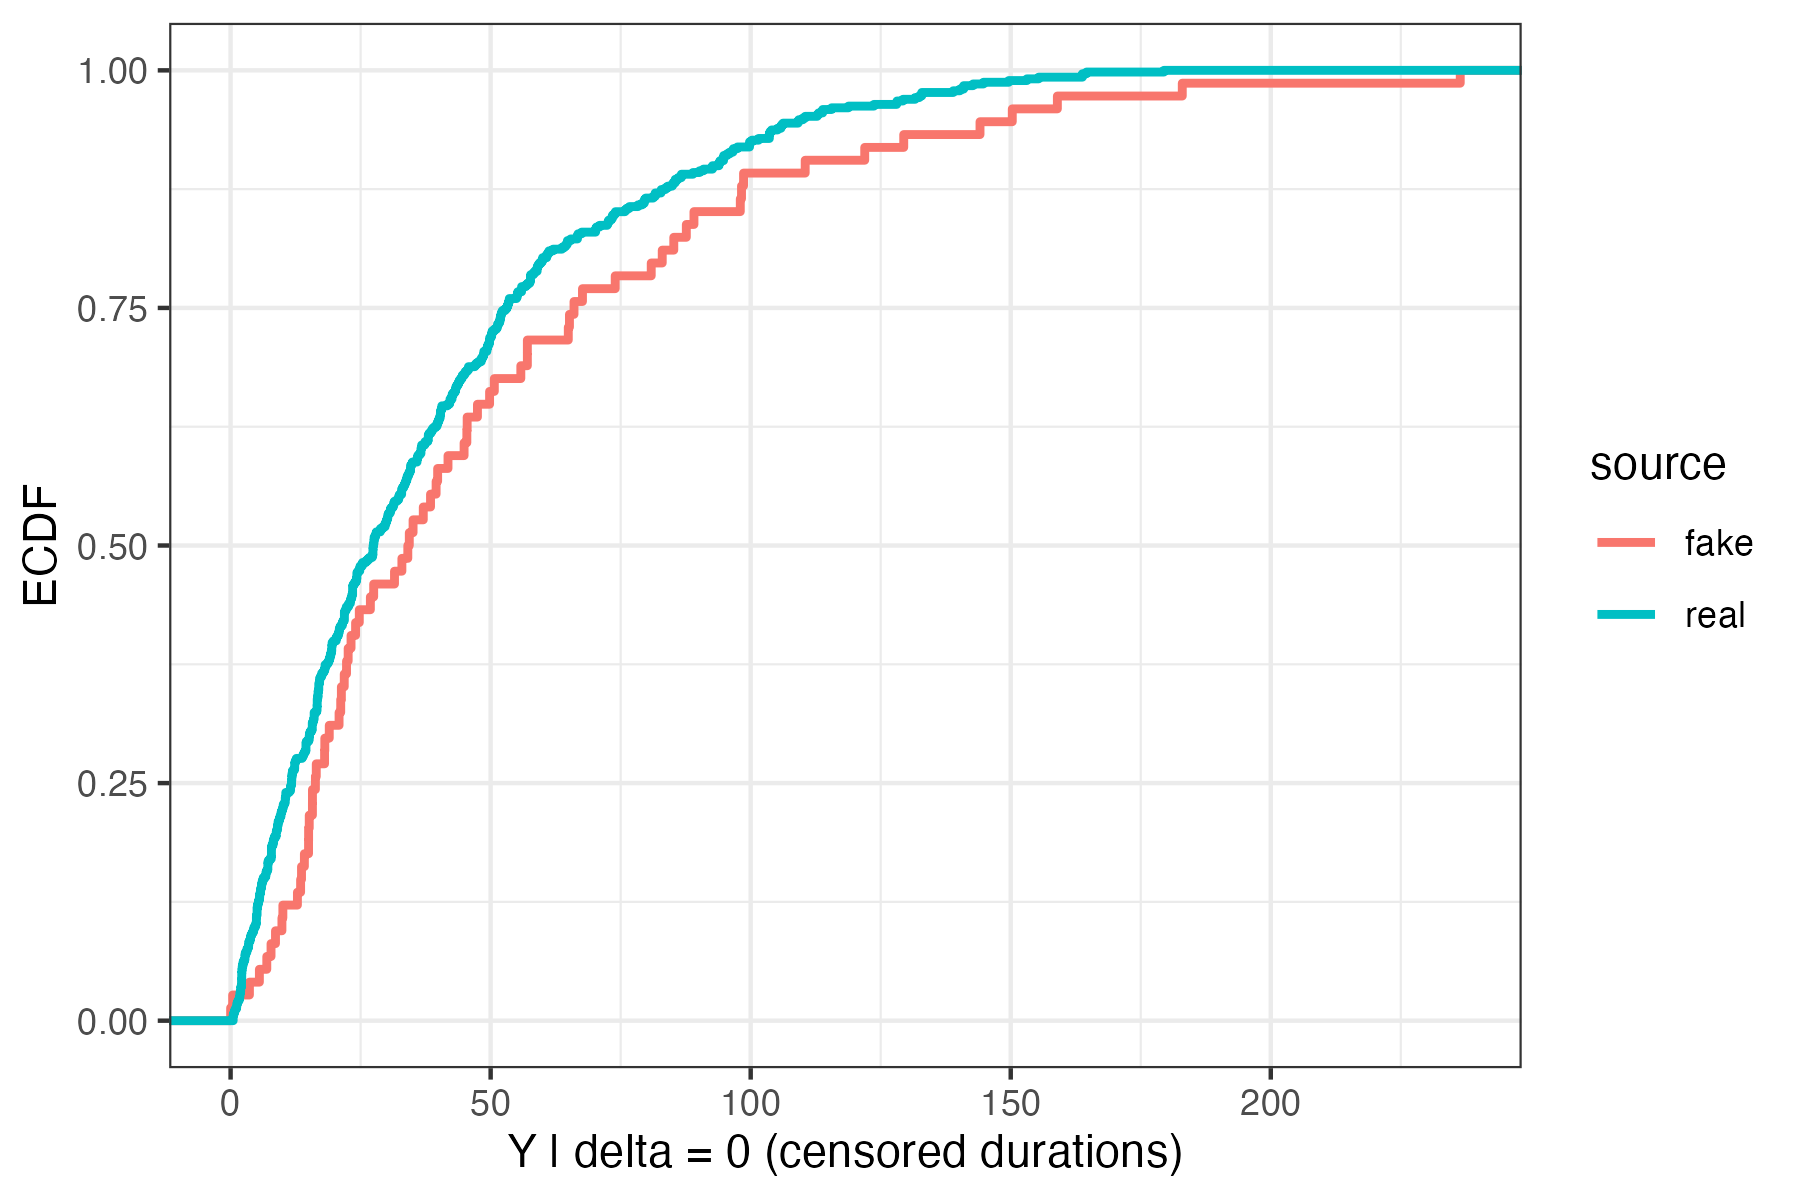
\includegraphics[width=\linewidth]{images/ppc_censored_ecdf_A1000.png} 
  \caption{{\small ECDF of $Y \mid \delta=0$}}
  \label{fig:ecdf-cens_a1000}
\end{subfigure}\hfill
\begin{subfigure}[t]{0.37\textwidth}
  \centering
  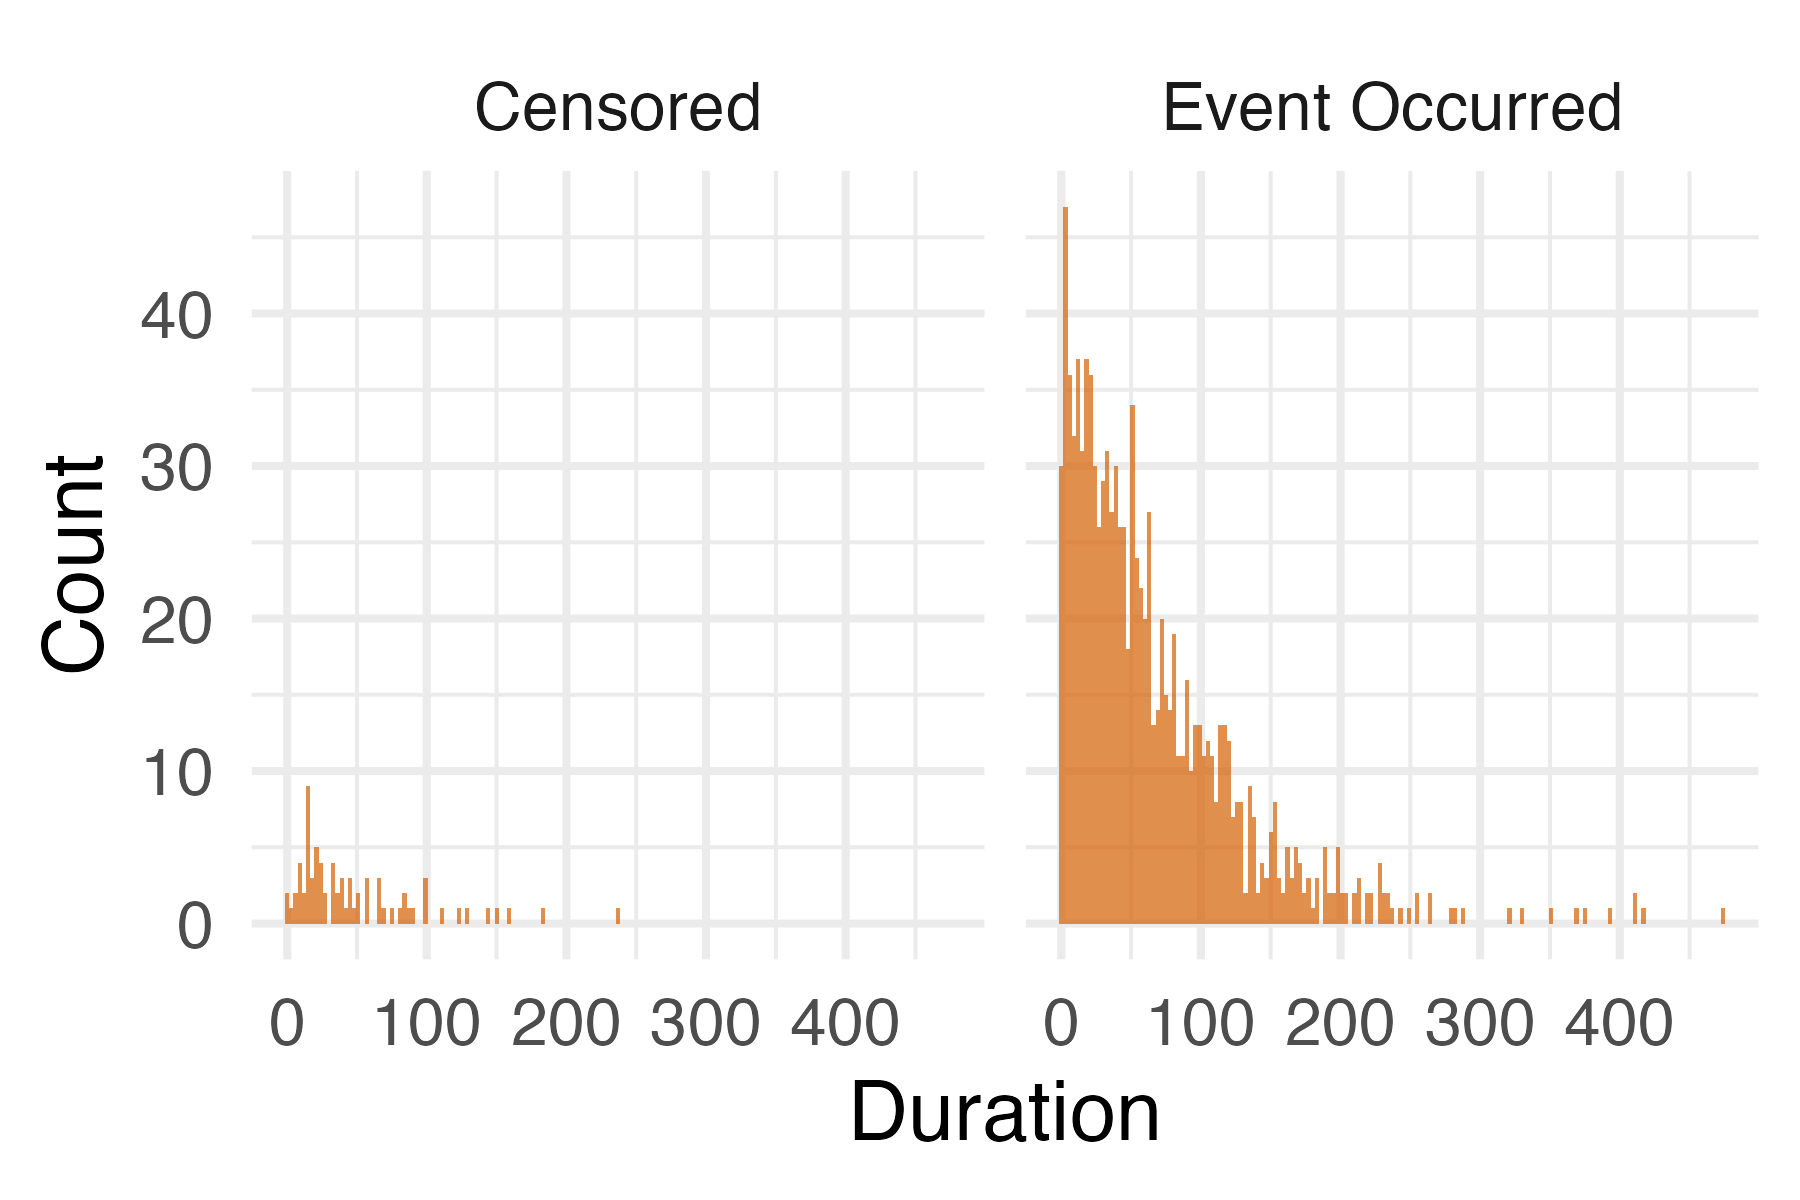
\includegraphics[width=\linewidth]{images/fake_duration_hist_a1000.png}   % 图3路径
  \caption{{\small Fake-data histogram}}
  \label{fig:fake-hist_a1000}
\end{subfigure}
\caption{{\small Posterior predictive checking ($A=1000$).}}
\label{fig:ppc-A1000}
\end{figure}
These examples underscore that posterior predictive fit must be interpreted in light of the plausibility of data-generating assumptions. Determining a realistic range for $A$ is essential for credible model checking, and this motivates the next step—explicitly incorporating $A$ into the likelihood and estimating it jointly with event-time parameters.


\subsection{Bayesian Estimation of \texorpdfstring{$A$}{A} in Exponential Censoring Models}
Building on the insights from the two extreme examples in Section~\ref{Impact of A}, we note that structural features of the censoring mechanism, such as a fixed observation window, can substantially influence parameter estimation. Such a structure is often overlooked in standard survival models, even though ignoring it may distort inference~\cite{bartovs2022informed,barrajón2020effectrightcensoringbias}. To address this, and while retaining the exponential event-time model introduced in Section~\ref{Exponential Model}, we introduce a global parameter $A$, defining the upper bound of the censoring time $C_i \sim \mathrm{Unif}(0, A)$~\cite{ibrahim2013bayesian}. This formulation more faithfully represents the data-generating process, facilitates objective simulation and model checking, and captures latent structures that are not directly observed but implicitly present. Although $A$ is unobserved in the data, it is identifiable under a Bayesian framework, and its posterior distribution can reflect the underlying data collection mechanism.

Below, we formulate a Bayesian inference framework under an exponential survival model with censoring window parameter $A$, and derive the corresponding full-sample likelihood. The model is defined as follows~\cite{ibrahim2013bayesian, bartovs2022informed, gelman1995bayesian},
\begin{enumerate}
    \item Event time (latent variable): $
    T_i \mid \lambda \sim \mathrm{Exp}(\lambda), 
    \qquad f_T(t \mid \lambda)=\lambda e^{-\lambda t},\; t\ge0.
    $
   \item Censoring time: $
   C_i \mid A \sim \mathrm{Unif}(0,A), 
   \qquad g_A(c)=\tfrac1A \mathbf 1\{0\le c\le A\}.
   $
   \item Independent censoring: $T_i \perp C_i \mid (\lambda, A).$
   \item Observed variables: $ Y_i=\min(T_i,C_i), \qquad 
   \delta_i=\mathbf 1\{T_i\le C_i\}.
   $
\end{enumerate}
Based on this setup, we derive the sample likelihood for each observation $(Y_i, \delta_i)$ under parameters $(\lambda, A)$, considering two possible observation types.

For event samples ($\delta_i=1,\, Y_i=y_i$), where the event occurs before censoring, i.e., $T_i = y_i,\; C_i \ge y_i$, the likelihood is
{\footnotesize
\begin{align}
p(y_i,\delta_i=1\mid\theta)
 &= \Pr\bigl(T_i=y_i,\,C_i\ge y_i \mid \theta\bigr) \\[3pt]
 &= \int_{c=y_i}^{A} \underbrace{p(T_i=y_i,\,C_i=c \mid \theta)}_{\text{joint density}}\,dc 
    &&\text{(marginalizing over unknown $C_i$~\cite{berger1999integrated})}\\
 &= \int_{y_i}^{A} f_T(y_i\mid\lambda)\,g_A(c)\,dc 
    && \text{ (by independence }T_i\perp C_i~\cite{sebastiani2008tutorial})\\
 &= f_T(y_i\mid\lambda)\,
    \bigl[\tfrac1A(A-y_i)\bigr]\,
    \mathbf 1\{0\le y_i\le A\}\\[3pt]
 &= \lambda e^{-\lambda y_i}\Bigl(1-\tfrac{y_i}{A}\Bigr)
    \mathbf 1\{0\le y_i\le A\}.
\end{align}}
For censored samples ($\delta_i=0,\, Y_i=y_i$), where censoring occurs before the event, i.e., $C_i = y_i,\; T_i > y_i$, the likelihood is
{\footnotesize
\begin{align}
p(y_i,\delta_i=0\mid\theta)
 &= \Pr\bigl(C_i=y_i,\,T_i>y_i \mid \theta\bigr) \\[0pt]
 &= \int_{t=y_i}^{\infty} 
    \underbrace{p(T_i=t,\,C_i=y_i \mid \theta)}_{\text{joint density}}\,dt
    &&\text{(marginalizing over unknown }T_i~\cite{berger1999integrated})\\[0pt]
 &= \int_{y_i}^{\infty} f_T(t\mid\lambda)\,g_A(y_i)\,dt
    &&\text{(factorized by independence~\cite{sebastiani2008tutorial})}\\[0pt]
 &= \frac{1}{A} \cdot \int_{y_i}^{\infty} f_T(t \mid \lambda) \, dt \cdot \mathbf{1}\{0 \le y_i \le A\} \\
 &= \frac{1}{A}\cdot \,S_T(y_i\mid\lambda)\,
    \mathbf 1\{0\le y_i\le A\}\\[3pt]
 &= \tfrac1A e^{-\lambda y_i}\mathbf 1\{0\le y_i\le A\},
\end{align}}
where $S_T(y\mid\lambda)=e^{-\lambda y}$ is the survival function of the exponential distribution.

Combining the two types of contributions, the full likelihood for the dataset $\mathcal{D} = \{(y_i, \delta_i)\}_{i=1}^n$ is
\begin{equation}
L(\mathcal{D}\mid\lambda,A)=
\prod_{i=1}^n
\bigl[\lambda e^{-\lambda y_i}(1-\tfrac{y_i}{A})\bigr]^{\delta_i}
\cdot \bigl[\tfrac{e^{-\lambda y_i}}{A}\bigr]^{1-\delta_i}
\cdot \mathbf 1\{0\le y_i \le A\}.
\label{A_likeli}
\end{equation}

Under the Bayesian framework, assuming independent priors $\pi_\lambda(\lambda)$ and $\pi_A(A)$, the joint posterior becomes
\begin{equation}
p(\lambda, A \mid \mathcal{D}) \propto 
L(\mathcal{D} \mid \lambda, A)\cdot
\pi_\lambda(\lambda)\cdot
\pi_A(A),
\qquad \text{with } A \ge \max_i y_i.
\label{A_post}
\end{equation}
This likelihood formulation explicitly incorporates the observation window as a structural parameter, improving transparency in the data-generating process and providing a foundation for subsequent posterior inference, prediction, and model checking~\cite{stats5010006}.



\subsection{Identifiability and Posterior Structure of \texorpdfstring{$\lambda$}{lambda} and \texorpdfstring{$A$}{A}}
After completing the Bayesian estimation for parameter $A$, a natural question arises: 
Does the extended survival model, under the parametrization $(\lambda, A)$, remain theoretically identifiable and consistent with the original exponential survival model?
To address this, we first establish the identifiability of $(\lambda, A)$ within this model, and then examine how the joint posterior structure and marginalization of $A$ reflect consistency with the baseline model. 

\subsubsection{Identifiability}
Once the new parameter $A$ is introduced, the first question is whether the model indexed by $(\lambda, A)$ remains identifiable. That is, whether distinct parameter values induce distinct distributions of the observables.
\begin{definition}\textbf{(Identifiability)}. Consider a statistical model $\mathcal P=\{P_\theta:\theta\in\Theta\}$, where $\theta$ is the parameter indexing the family and $\Theta$ may be finite- or infinite-dimensional. We say that $\mathcal P$ is identifiable under the parametrization $\theta$ if the following condition holds~\cite{lehmann1998theory, van2000asymptotic}
\begin{equation}
    P_{\theta_1}=P_{\theta_2}\ \Longrightarrow\ \theta_1=\theta_2,\qquad \forall\,\theta_1,\theta_2\in\Theta .
\end{equation}
Equivalently, the mapping $\theta\mapsto P_\theta$ is injective~\cite{lehmann1998theory}.
\end{definition}
%%%%%%%%%%%%%%%%%%%%%%%%%%%%%%%%
\begin{proof}
The observed data are pairs $(Y,\delta)$ with $Y=\min(T,C)$ and $\delta=\mathbf 1\{T\le C\}$. 
Under $T\sim\text{Exp}(\lambda)$, independent censoring with horizon $A$, and uniform entry, 
the distribution $P_\psi$ with $\psi=(\lambda,A)$ is characterized by two component densities
\begin{equation}
f_0(y\mid\lambda,A)=\frac{1}{A}\,e^{-\lambda y}, \quad 0\le y\le A, \qquad (\delta=0),
\end{equation}
\begin{equation}
f_1(y\mid\lambda,A)=\lambda e^{-\lambda y}\Big(1-\tfrac{y}{A}\Big), \quad 0<y<A, \qquad (\delta=1).
\end{equation}
\textbf{Identifiability of $A$}. 
For censored observations $(\delta=0)$, the density $f_0$ has support $[0,A]$, depending only on $A$. Suppose $P_{\lambda_1,A_1}=P_{\lambda_2,A_2}$. If $A_1\ne A_2$, without loss of generality let $A_1<A_2$, 
and consider $B=(A_1,(A_1+A_2)/2]$. Then
\begin{equation}
P_{\lambda_1,A_1}(Y\in B,\delta=0)=\int_B \tfrac{1}{A_1}e^{-\lambda_1 y}\,dy=0,
\end{equation}
while
\begin{equation}
P_{\lambda_2,A_2}(Y\in B,\delta=0)=\int_B \tfrac{1}{A_2}e^{-\lambda_2 y}\,dy>0.
\end{equation}
This contradiction implies $A_1=A_2$. Hence, the parameter $A$ is identifiable.

\textbf{Identifiability of $\lambda$.}
Fixing $A$, the support is identical across all parameter values, so differences must arise from the shape of the distribution. Since $P_\psi$ is fully determined by the pair $(f_0,f_1)$, any functional transformation thereof also characterizes the model. In particular, the ratio of event to censoring densities,
\begin{equation}
R(y;\lambda,A)=\frac{f_1(y\mid\lambda,A)}{f_0(y\mid\lambda,A)}=\lambda(A-y), \qquad 0<y<A ,
\end{equation}
provides a convenient summary to examine the role of $\lambda$. This ratio is a deterministic linear function in $y$, with slope $-\lambda$ and intercept $\lambda A$. Since $A$ has already been identified in step 1, equality of ratios implies $\lambda_1=\lambda_2$. 

Therefore, both parameters are uniquely determined by the distribution of $(Y,\delta)$, and the model is identifiable in $(\lambda,A)$.
\end{proof}

\subsubsection{Grid-based Contour Analysis of the Joint Posterior}

To further examine how identifiability appears in finite-sample settings, we characterize the shape of the joint posterior distribution and visualize its structure numerically.

As shown in Equation~\eqref{A_post} of Section~\ref{A_bayes}, we adopt the same prior for $\lambda$ as in Section~\ref{指数模型贝叶斯推断过程} (the exponential model case), to ensure comparability and to facilitate the later marginalization check in Section~\ref{边际化章节}. For $A$, we use a uniform prior $\mathrm{Unif}(y_{\max}, y_{\max}+500)$, which is relatively broad but still consistent with the constraints discussed in Section~\ref{Impact of A}: the survey duration cannot extend indefinitely (e.g., 1000 months).

Under this setting, the log-posterior is
\begin{align}
\log p(\lambda, A \mid \mathcal D)
&= \text{const}
   + \Big(\sum_{i=1}^n \delta_i\Big)\log \lambda
   - \lambda \sum_{i=1}^n y_i \nonumber\\[6pt]
&\quad + \sum_{i:\,\delta_i=1}\log(A-y_i)
   - n \log A
   + \log \pi_\lambda(\lambda) \nonumber \\[6pt]
&\quad + \log \pi_A(A) + \log \mathbf 1\{A \ge \max_i y_i\}.
\end{align}
Since the model involves only two parameters $(\lambda, A)$, we approximate the posterior on a two-dimensional grid~\cite{mcelreath2021grid}. At each grid point $(\lambda_i, A_j)$, we evaluate the log-posterior, exponentiate, and normalize to obtain weights~\cite{ORMEROD201145,mcelreath2021grid}
\begin{equation}
    w_{ij} \;\propto\; \exp\!\Bigl(\log p(\lambda_i, A_j \mid \mathcal D)\Bigr), \qquad \tilde w_{ij} \;=\; \frac{w_{ij}}{\sum_{i,j} w_{ij}} ,
\end{equation}
which provides a discrete approximation to the posterior distribution.

Based on these weights, the geometry of the posterior can be visualized directly using contour plots~\cite{maclaren2020estimatedidentifiabilityestimabilitycausal, mcelreath2021grid}. Unlike MCMC, this grid-based approach avoids issues of convergence diagnostics, while the two-dimensional grid enables a complete visualization of the posterior structure~\cite{joshi2016improvinggridbasedbayesian} (e.g., unimodality, multimodality, tail behaviour). This helps to reveal parameter dependencies and assess finite-sample identifiability.

In addition to raw contour visualization, we compute highest posterior density (HPD) regions on the grid, corresponding to coverage levels analogous to one- and two-standard-deviation intervals under a Gaussian distribution (39.3\% and 86.5\%)~\cite{kocev2021modeling}. These HPD contours provide a quantitative summary of posterior uncertainty, enabling us to assess whether the joint posterior exhibits approximately normal behavior or deviates substantially (e.g., through skewness or heavy tails).
\begin{figure}[H]
    \centering
    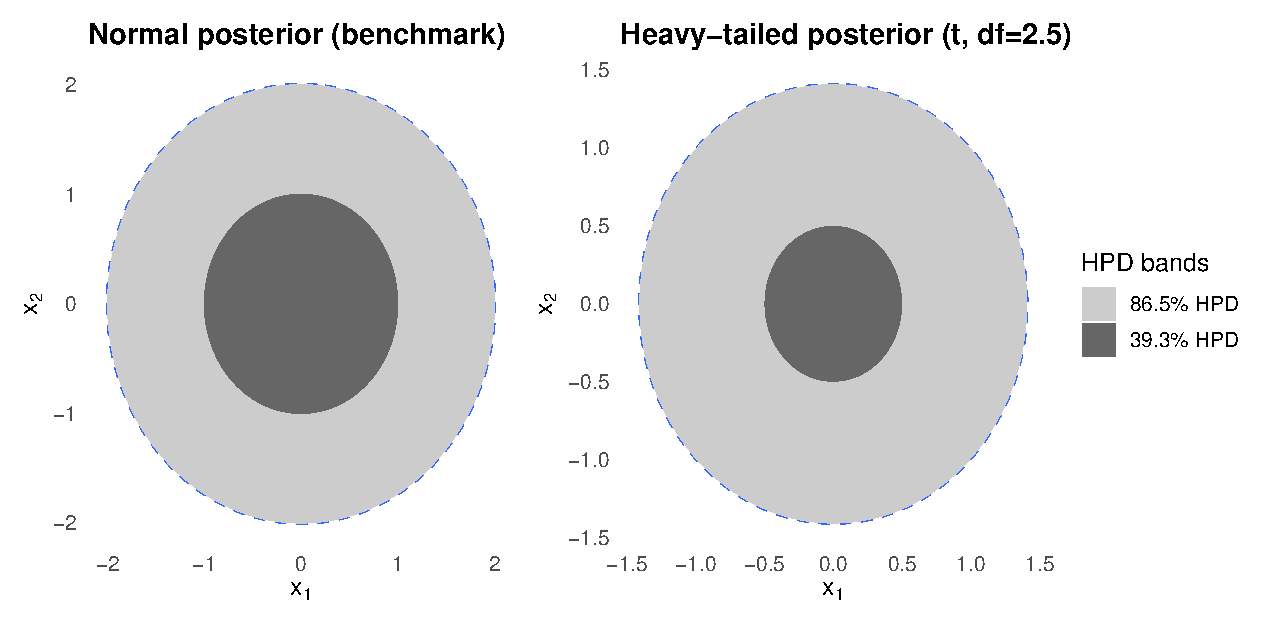
\includegraphics[height=5.5cm, width=0.8\textwidth]{images/hpd_normal_vs_student-t.pdf}
    \caption{{\small Illustrative HPD regions (39.3\% and 86.5\%) under a bivariate normal posterior (left) and a heavy-tailed $t$ distribution ($\text{df}=2.5$, right), both with $\mu=(0,0)$ and $\Sigma=I_2$.}}
    \label{fig:hpd-example}
\end{figure}
After obtaining the discretised posterior distribution, a natural next step is to extract the maximum a posteriori (MAP) estimate~\cite{gelman1995bayesian}. Within the grid framework, the MAP corresponds to the grid point $(\lambda^*, A^*)$ with the highest weight
\begin{equation}
    (\lambda^*, A^*) = \arg\max_{\lambda,A} \; p(\lambda,A \mid \mathcal D).
\end{equation}
This provides the most plausible parameter pair, which can serve as a reference point for pseudo-data generation and subsequent model checking~\cite{robert2007bayesian, gelman1995bayesian}.



\subsubsection{Marginalization of \texorpdfstring{$A$}{A} and Consistency Check}
\label{边际化章节}
The joint posterior $p(\lambda, A \mid \mathcal D)$ captures the dependence between the two parameters. To verify theoretical consistency with the original exponential model, we consider the marginal posterior of $\lambda$ obtained by integrating out $A$~\cite{gelman1995bayesian}.   

The central question is: does the marginal posterior of $\lambda$ coincide with that of the original exponential model (Equation~\ref{eq:16})? If so, this confirms that the extended model remains compatible with the original formulation and does not alter inference on $\lambda$.

Starting from Equation~\eqref{A_post}, we integrate out $A$~\cite{berger1999integrated}
\begin{equation}
    p(\lambda \mid \mathcal D)
= \int p(\lambda, A \mid \mathcal D)\,dA.
\end{equation}
Substituting, we obtain
\begin{equation}
    p(\lambda \mid \mathcal D)\;\propto\;\pi_\lambda(\lambda)\;\int L(\mathcal D \mid \lambda, A)\,\pi_A(A)\,dA.
    \label{eq:45}
\end{equation}
Thus, the integral in~\eqref{eq:45} reduces to a constant term independent of $\lambda$. 
Importantly, this constant absorbs both the $A$-dependent part of the likelihood and the prior $\pi_A(A)$, which means that the marginal posterior of $\lambda$ is independent of the prior choice for $A$. 
Therefore,
\begin{equation}
    L(\mathcal D \mid \lambda, A)
= \lambda^{\sum_i \delta_i}\;
e^{-\lambda \sum_i y_i}\;
\Bigg[
A^{-n}\,\prod_{i:\,\delta_i=1}(A-y_i)
\Bigg]\;\mathbf 1\{A \ge \max_i y_i\}.
\end{equation}
the integral in~\eqref{eq:45} separates into a constant term independent of $\lambda$. Thus,
\begin{align}
\label{eq:47}
p(\lambda \mid \mathcal{D})
&\propto \lambda^{\sum_i \delta_i}\,
e^{-\lambda \sum_i y_i}\,
\pi_\lambda(\lambda)\,
\underbrace{\int_{A \ge \max_i y_i}
A^{-n}\,\prod_{i:\,\delta_i=1}(A-y_i)\,\pi_A(A)\,dA}_{\text{constant, independent of }\lambda} \\[2pt]
&\propto \lambda^{\sum_i \delta_i}\, e^{-\lambda \sum_i y_i}\, \pi_{\lambda}(\lambda).
\end{align}
This is exactly the posterior distribution of the original exponential model (Equation~\ref{eq:16}).  

Numerically, the same result can be recovered by marginalizing over $A$ in the grid-based posterior representation: summing the normalized weights $\tilde w_{ij}$ along the $A$ dimension for each fixed $\lambda$ yields the marginal posterior of $\lambda$~\cite{ORMEROD201145, cowles2009reparameterized}. This numerical implementation matches the analytical derivation above, providing a computational-theoretical cross-check.

In summary, marginalizing $A$ restores the same posterior distribution for $\lambda$ as in the original exponential model. This demonstrates that the extended model is fully consistent with the original formulation: introducing $A$ enriches the model by explicitly representing the censoring window, while preserving the fundamental inference on $\lambda$.














